\documentclass{beamer}

\usepackage{amsmath}
\usepackage{booktabs} % Para tabelas com visual profissional
\usepackage{tabularx} % Para tabelas com largura definida e colunas do tipo X


\usetheme{Madrid}
\usecolortheme{beaver}
\usepackage[utf8]{inputenc}
\usepackage[brazil]{babel}
\usepackage{graphicx}
\usepackage{xcolor}
\usepackage{colortbl} % para sombrear células da tabela
\usepackage{tikz}
%\usetikzlibrary{shapes, arrows.meta, positioning}
\usetikzlibrary{shapes.geometric, arrows.meta, positioning}

\usepackage{array} 

\usepackage{tcolorbox}     % Para caixas coloridas e formatadas
\tcbuselibrary{skins, breakable}  % Habilita opções avançadas do tcolorbox
\usepackage{graphicx}      % Necessário para \scalebox
\usepackage{hyperref}
\hypersetup{
    colorlinks=true,
    %linkcolor=blue,
    filecolor=magenta,      
    urlcolor=cyan,
    pdfpagemode=FullScreen,
    }

\urlstyle{same}


\definecolor{graycell}{gray}{0.85} % define a cor de fundo da célula
\definecolor{vermelhoClaro}{RGB}{255, 200, 200}


\AtBeginSection[]
{
  \begin{frame}
    \frametitle{Índice}
    \tableofcontents[currentsection]
  \end{frame}
}

%% Placeholder para figuras ainda não disponíveis: se o arquivo existir em img/,
%% inclui a imagem; senão desenha uma caixa indicando qual figura do livro buscar.
%% Uso: \figuraplaceholder[largura]{img/arquivo.png}{Fig. X.Y do livro (pág. Z)}
\newcommand{\figuraplaceholder}[3][0.8\textwidth]{%
    \IfFileExists{#2}{%
        \includegraphics[width=#1]{#2}%
    }{%
        \begin{tikzpicture}
            \node[draw=gray!70, dashed, very thick, fill=gray!10,
                  minimum width=0.85\textwidth, minimum height=2.6cm, align=center]
                {{\large\bfseries\color{gray!60!black} PLACEHOLDER}\\[3pt]
                 #3\\[3pt]
                 {\footnotesize arquivo esperado: \texttt{#2}}};
        \end{tikzpicture}%
    }%
}

% Informações da apresentação
\title[Funções Hash]{Funções Hash}
\author{Prof. Iaçanã Ianiski Weber}
\institute{PUCRS}
\date{CSS (98G08-4)}

\begin{document}

% Slide de Capa Personalizado
\begin{frame}[plain]

% Linha superior com logo e título
\noindent
\begin{minipage}[t]{0.15\textwidth}
    
\includegraphics[width=\linewidth]{img/Brasão_PUCRS.png}
\end{minipage}%
\begin{minipage}[t]{0.84\textwidth}
    \begin{center}
        \raisebox{2ex}{\LARGE\bfseries\textcolor{blue} {\textbf{Funções Hash}}}\\
    \end{center}
\end{minipage}

\vspace{2cm}

\begin{center}
    \Large \textbf{Prof. Dr. Iaçanã Ianiski Weber} \\
    \vspace{0.2cm}
    \normalsize \textit{Confiabilidade e Segurança de Software} \\
    \vspace{0.2cm}
    \large 98G08-4
\end{center}

\vfill

\begin{center}
    \tiny \textit{Agradecimentos especiais ao Prof. Avelino Zorzo e aos Autores Christof Paar e Jan Pelzl pelo material.}
\end{center}

\end{frame}

% Slide de Índice
\begin{frame}{Índice}
    \tableofcontents
\end{frame}

%%%%%%%%%%%%%%%%%%%%%%%%%%%%%%%%%%%
%%%%%%%%%%%%%%%%%%%%%%%%%%%%%%%%%%%
%%%%%%%%%%%%%%%%%%%%%%%%%%%%%%%%%%%
\section{Porque Precisamos de Funções Hash}

\begin{frame}{Motivação}
    \frametitle{Por que usar Funções de Hash para Assinaturas?}
    \vspace{-0.5em}
    \textbf{O Problema: Assinatura ingênua de mensagens longas}
    
    \small{Assinar uma mensagem longa em blocos separados gera uma assinatura de tamanho similar ao da própria mensagem, o que é ineficiente.}

    \begin{figure}
        \centering
        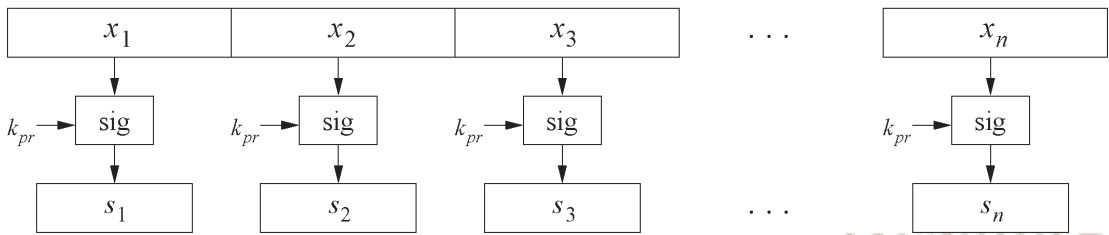
\includegraphics[width=0.75\textwidth]{naive_sign.png}
    \end{figure}

    \begin{columns}[T]
        \footnotesize
        \begin{column}{0.55\textwidth}
            \textbf{Isto gera três problemas principais:}
            \begin{itemize}
                \item \textbf{Sobrecarga Computacional:} Operações de chave pública são lentas e custosas para cada bloco.
                \item \textbf{Sobrecarga de Mensagem:} A assinatura final fica muito grande.
                \item \textbf{Limitações de Segurança:} Um atacante pode reordenar, remover ou duplicar blocos para forjar novas mensagens.
            \end{itemize}
        \end{column}

        \begin{column}{0.45\textwidth}
            {\large\textbf{\color{blue!70!black}Solução}}
            \vspace{0.5em}
            
            Em vez de assinar a mensagem inteira, assina-se apenas seu \textbf{digest} (ou \textbf{hash}).
            \begin{itemize}
                \item[$\rightarrow$] Igualmente seguro, muito mais rápido.
            \end{itemize}
            
            \vspace{1.2em}
            {\large\textbf{\color{green!60!black}Necessidade}}
            \vspace{0.5em}
            
            % O comando \normalsize foi removido daqui.
            Isso requer o uso de \textbf{Funções de Hash} criptográficas.

        \end{column}
    \end{columns}
\end{frame}

\begin{frame}{Assinatura Digital com Função Hash}

\begin{figure}
    \centering
    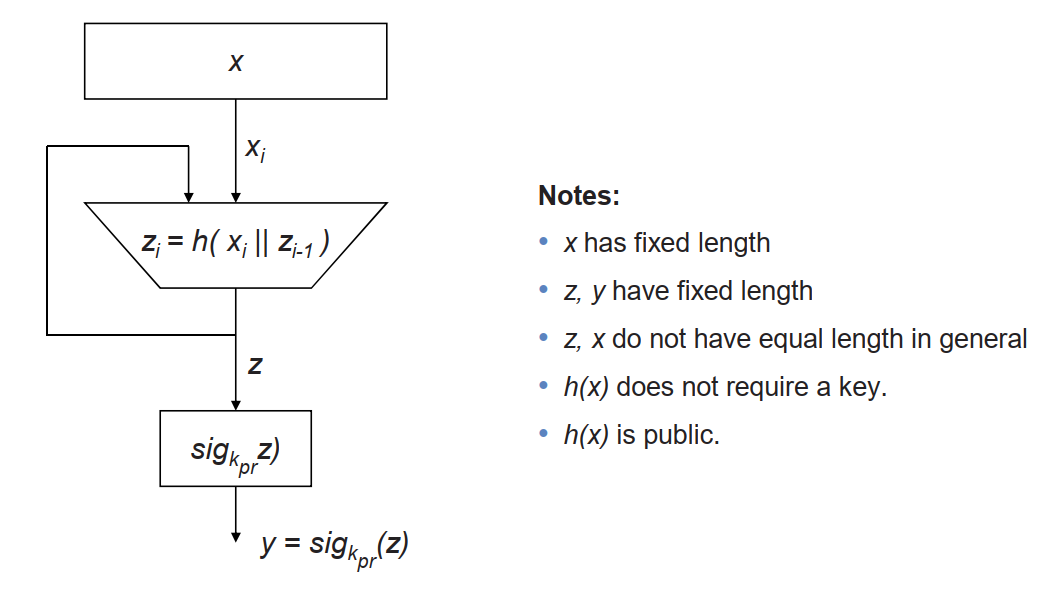
\includegraphics[width=1\linewidth]{sign_with_hash.png}
\end{figure}
    
\end{frame}

\begin{frame}{Protocolo Básico de Assinatura Digital usando Função Hash}

\begin{figure}
    \centering
    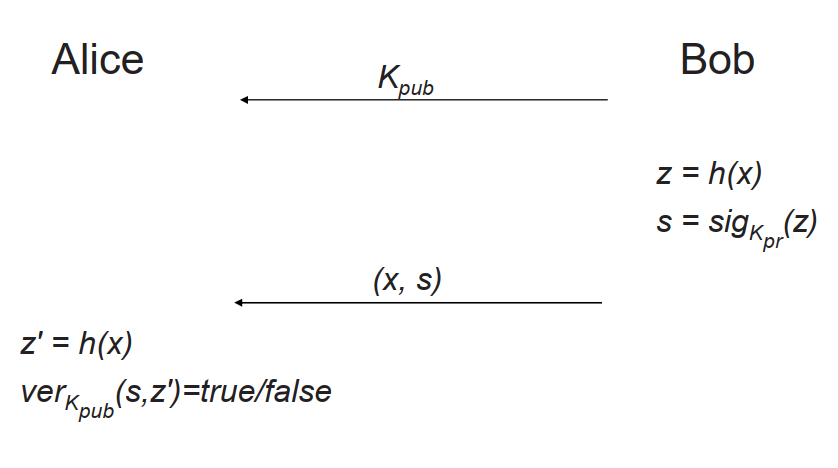
\includegraphics[width=1\linewidth]{basic_protocol_sign_with_hash.png}
\end{figure}

\end{frame}

\section{Propriedades de Funções de Hash}

\begin{frame}{Propriedades de Funções de Hash}
    \frametitle{O que uma Função de Hash faz?}
    
    \centering
    
    \resizebox{0.75\textwidth}{!}{%
        \begin{tikzpicture}[
            node distance=0.4cm and 1.2cm,
            caixa_msg/.style={
                draw, rectangle, rounded corners, fill=blue!10,
                minimum height=1.2cm, text width=5.5cm, align=center
            },
            caixa_hash/.style={
                draw, rectangle, rounded corners, fill=green!10, font=\ttfamily,
                minimum height=1.2cm, text width=3.5cm, align=center
            },
            seta/.style={->, thick, draw=gray!80}
        ]
            % Rótulos das colunas
            \node (msg_label) at (0,0) {\textbf{Mensagem (\textit{x})}};
            \node[right=of msg_label, xshift=4cm] (hsh_label) {\textbf{Digest (\textit{y = h(x)})}};

            % --- Exemplo 1: Texto longo ---
            % =================================================================
            % AQUI ESTÁ A CORREÇÃO DEFINITIVA USANDO UMA \parbox
            % =================================================================
            \node[caixa_msg, below=of msg_label] (m1) {\parbox{5.5cm}{\centering Toda história de amor começa com ``era uma vez\dots''{,}` exceto a de Alice e Bob{,}` que começa com ``gerei uma chave pública''.}};
            
            \node[caixa_hash, right=of m1, xshift=2.5cm] (h1) {xDFDC349A23};
            \draw[seta] (m1) -- node[above, sloped] {h(x)} (h1);

            % --- Exemplo 2: Texto curto (com a frase engraçada) ---
            \node[caixa_msg, below=of m1] (m2) {Ela viu o pai.};
            \node[caixa_hash, right=of m2, xshift=2.5cm] (h2) {xA3F4439B1E};
            \draw[seta] (m2) -- node[above, sloped] {h(x)} (h2);

            % --- Exemplo 3: Uma chave ---
            \node[caixa_msg, below=of m2] (m3) {Ela viu o par.};
            \node[caixa_hash, right=of m3, xshift=2.5cm] (h3) {xFB93E283A1};
            \draw[seta] (m3) -- node[above, sloped] {h(x)} (h3);

        \end{tikzpicture}%
    } % Fim do \resizebox

    % Lista de propriedades
    \begin{itemize}
    \small
        \item \textbf{Entrada de tamanho arbitrário:} A função $h$ opera sobre uma mensagem $x$ de qualquer comprimento.
        \item \textbf{Saída de tamanho fixo:} O resultado (digest) $y=h(x)$ tem sempre o mesmo comprimento (ex: 256 bits).
        \item \textbf{Função de mão única (\textit{one-way}):} Dado $x$, é fácil computar $h(x)$. Dado $h(x)$, é computacionalmente inviável encontrar $x$.
    \end{itemize}
\end{frame}

\begin{frame}{As três propriedades das Funções Hash}

\begin{figure}
    \centering
    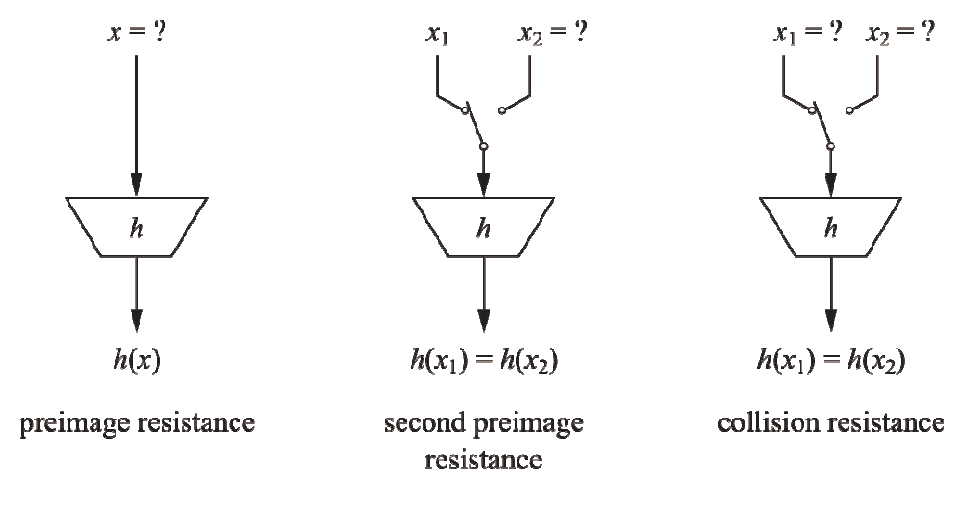
\includegraphics[width=1\linewidth]{tres_propriedades.png}
\end{figure}
    
\end{frame}

\begin{frame}{Funções de Hash: Propriedades de Segurança}
    \frametitle{As Três Garantias Fundamentais}

    \begin{itemize}
        \item \textbf{Resistência à pré-imagem (\textit{Preimage resistance})} \medskip\\
        Para uma dada saída $z$, é computacionalmente inviável encontrar qualquer entrada $x$ tal que $h(x) = z$.
        \vspace{0.5em}
        \begin{itemize}
        \footnotesize
            \item Essencialmente, a propriedade de ser uma função de \alert{mão única (\textit{one-way})}.
        \end{itemize}
        \bigskip

        \item \textbf{Resistência à segunda pré-imagem (\textit{Second preimage resistance})} \medskip\\
        Dado um bloco de dados $x_1$, é computacionalmente inviável encontrar \textit{outro} bloco $x_2$ tal que $x_1 \neq x_2$ e que $h(x_1) = h(x_2)$.
        \vspace{0.5em}
        \begin{itemize}
            \item Protege contra a falsificação de um documento já assinado.
        \end{itemize}
        \bigskip

        \item \textbf{Resistência à colisão (\textit{Collision resistance})} \medskip\\
        É computacionalmente inviável encontrar \textit{qualquer par} de entradas distintas $x_1, x_2$ tal que $x_1 \neq x_2$ e que $h(x_1) = h(x_2)$.
        \vspace{0.5em}
        \begin{itemize}
            \item É uma propriedade mais forte que a resistência à segunda pré-imagem.
        \end{itemize}

    \end{itemize}
\end{frame}

\begin{frame}{Funções de Hash e o Problema da Colisão}
    \frametitle{O Paradoxo do Aniversário}

    \begin{itemize}
        \item A \textbf{resistência à colisão} é a propriedade que, na prática, causa mais problemas de segurança. \pause
        
        \bigskip
        \item \textbf{Pergunta análoga:} Quantas pessoas são necessárias em uma sala para que a probabilidade de duas delas fazerem aniversário no mesmo dia seja de 50\%? \pause
        
        \begin{itemize}
            \item A resposta intuitiva seria 365/2 $\approx$ 183? \pause \alert{Não!}
        \end{itemize}
        
        \bigskip
        \item Apenas \alert{23 pessoas} são suficientes! Isso é conhecido como o \textbf{Paradoxo do Aniversário}. \pause
        
        \bigskip
        \item \textbf{Implicação para Hashes:} Um ataque para encontrar colisões (chamado de \textit{birthday attack}) é muito mais eficiente do que um ataque de força bruta. A busca leva aproximadamente $2^{n/2}$ passos para uma função de hash com saída de $n$ bits. \pause

        
    \end{itemize}
\end{frame}

\begin{frame}{O Paradoxo do Aniversário}
        \textbf{Por que o paradoxo funciona?}
        \begin{itemize}
        \footnotesize
            \item A intuição falha porque não consideramos o número de \textbf{pares} possíveis. Com apenas 23 pessoas, existem 253 pares distintos, aumentando drasticamente a chance de uma coincidência.
            \item Em um ataque, o atacante não precisa quebrar o hash de um documento específico. Ele pode gerar várias versões de um documento bom e de um malicioso até que \textit{qualquer par} entre eles produza o mesmo hash, o que é um problema muito mais fácil de resolver.
        \end{itemize} \pause

        \bigskip
        \textbf{Recomendação de Segurança:} Para se proteger deste ataque, a recomendação é que a saída de uma função de hash deve ter \textbf{no mínimo 224 bits}.

\end{frame}

\begin{frame}{O Paradoxo do Aniversário em Números}
    \begin{center}
        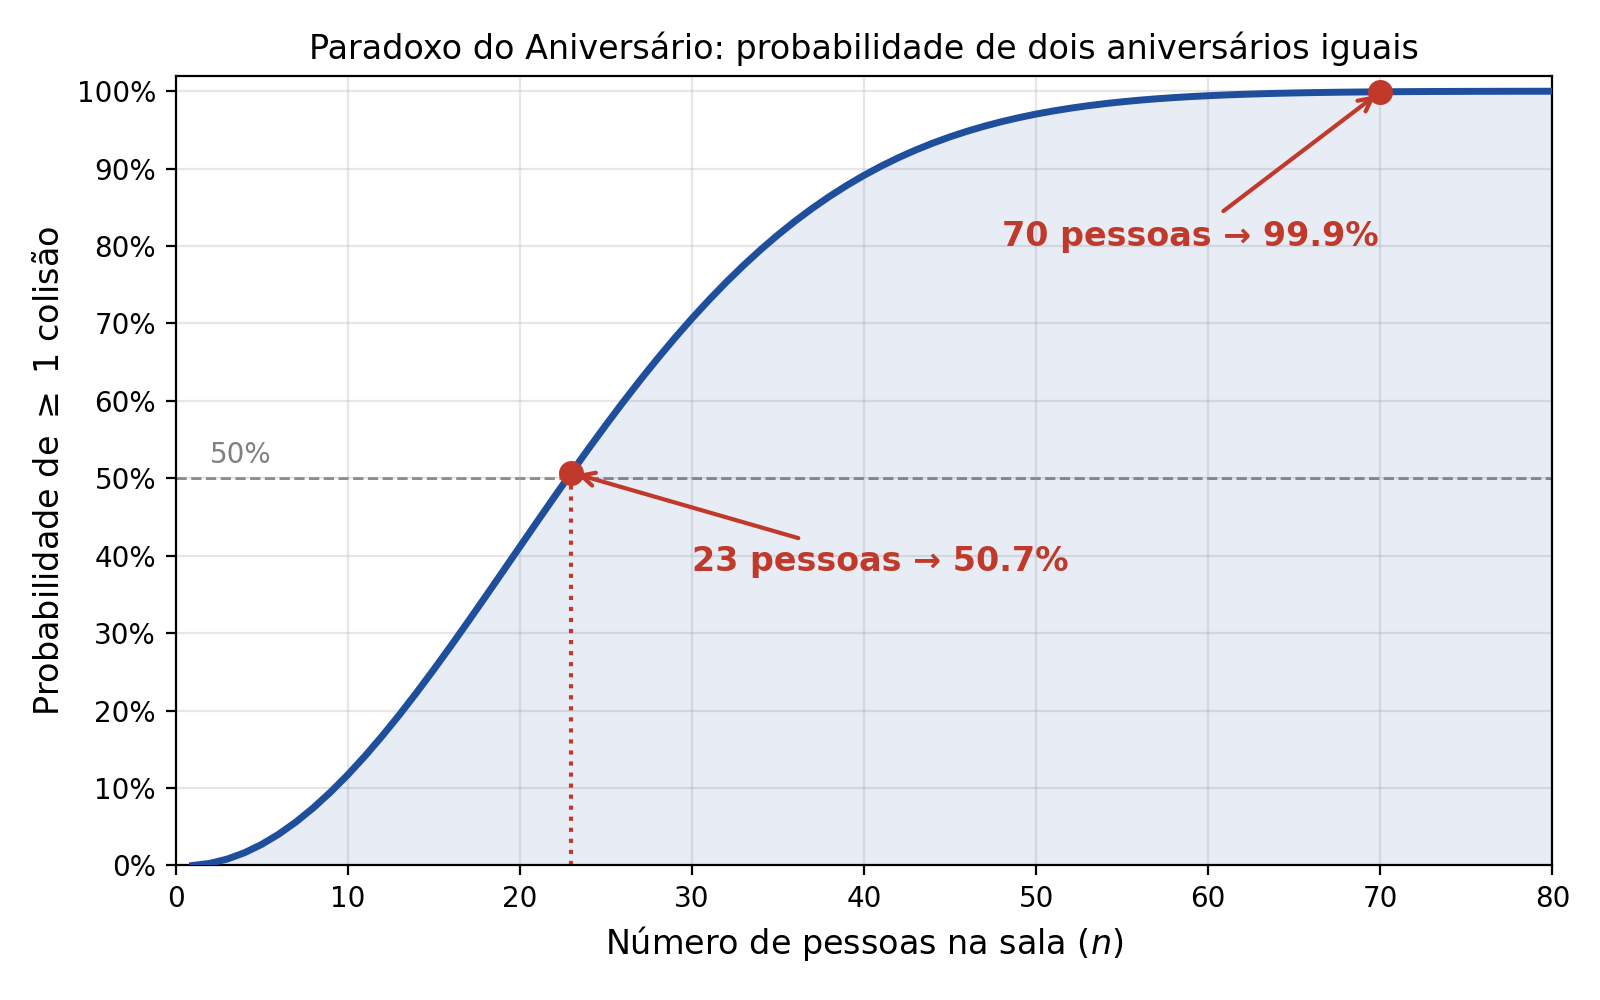
\includegraphics[width=0.78\textwidth]{img/birthday_paradox.png}
    \end{center}
    \begin{itemize}
        \footnotesize
        \item A curva sobe muito mais rápido do que a intuição sugere: com 23 pessoas ($\approx 6\%$ dos 365 dias!) a colisão já é mais provável que não, pois o número de \textbf{pares} cresce como $\binom{n}{2}$.
        \item Para funções de hash vale o mesmo: com $\approx \sqrt{2^n} = 2^{n/2}$ tentativas, encontrar \textit{alguma} colisão torna-se provável: é o \textit{birthday attack}.
    \end{itemize}
\end{frame}

\begin{frame}{O Ataque de Aniversário e a Segurança Moderna}

    \begin{itemize}
        \item O \textbf{Paradoxo do Aniversário} mostra que é muito mais fácil encontrar \textit{qualquer} colisão do que uma específica.
        \begin{itemize}
            \item Para um hash de $n$ bits, a complexidade de um ataque de aniversário é de aproximadamente $2^{n/2}$ operações.
        \end{itemize}
        
        \bigskip
        \item \textbf{O Padrão Antigo (Obsoleto)}
        \begin{itemize}
            \item A recomendação de 160 bits (do algoritmo SHA-1) oferecia $160/2 = 80$ bits de segurança contra colisão.
            \item Este nível de segurança ($2^{80}$) \alert{não é mais considerado seguro} contra adversários com recursos significativos.
        \end{itemize}

        \bigskip
        \item \textbf{A Recomendação Atual (NIST)}
        \begin{itemize}
            \item O NIST exige um nível de segurança de no mínimo \textbf{112 bits} contra colisão.
            \item Para isso, a saída do hash deve ter no mínimo $2 \times 112 = \textbf{224 bits}$.
        \end{itemize}

        \bigskip
        \item \textbf{Conclusão Prática para Novos Sistemas:}
        \begin{itemize}
            \item<2-> \alert{Use no mínimo SHA-256} (saída de 256 bits).
            \item<2-> Abandone completamente o uso de SHA-1.
        \end{itemize}
    \end{itemize}
\end{frame}

%\section {Algorítmos}
\begin{frame}{Funções de Hash: Lições Aprendidas}

    \begin{itemize}
        \small
        \item \textbf{Natureza e Uso Principal}
        \small
        \begin{itemize}
            \item Funções de Hash não usam chaves (\textit{keyless}).
            \item Suas aplicações mais importantes são em assinaturas digitais e em códigos de autenticação de mensagens (MACs), como o HMAC.
        \end{itemize}
        
        \item \textbf{Requisitos de Segurança Fundamentais}
        \small
        \begin{itemize}
            \item As três propriedades de segurança essenciais são a resistência à pré-imagem (one-wayness), à segunda pré-imagem e à colisão.
        \end{itemize}

        \item \textbf{Estado Atual dos Algoritmos}
        \small
        \begin{itemize}
            \item \textbf{MD5 e SHA-1:} São considerados \alert{inseguros}. O SHA-1 possui falhas graves e seu uso deve ser completamente descontinuado.
            \item \textbf{SHA-2:} A família de algoritmos SHA-2 (ex: SHA-256, SHA-512) continua sendo considerada segura e é o padrão de mercado atual.
            \item \textbf{SHA-3 (Atualização):} A competição SHA-3 \alert{terminou em 2012}. O algoritmo vencedor (Keccak) foi padronizado em 2015. Ele serve como uma alternativa moderna ao SHA-2.
        \end{itemize}

        
        \item \textbf{Recomendação de Tamanho (Atualizada)}
        \small
        \begin{itemize}
            \item Para segurança de longo prazo e para resistir a ataques de colisão (ataques de aniversário), a recomendação atual é usar saídas de no mínimo \alert{256 bits}.
        \end{itemize}
    \end{itemize}
\end{frame}

%%%%%%%%%%%%%%%%%%%%%%%%%%%%%%%%%%%
%%%%%%%%%%%%%%%%%%%%%%%%%%%%%%%%%%%
%%%%%%%%%%%%%%%%%%%%%%%%%%%%%%%%%%%
\section{SHA-2}

\begin{frame}{De MD4 ao SHA-2: Uma Breve História}
    \textbf{SHA-2 não nasceu do zero}: ele é o integrante mais bem-sucedido da \textbf{família MD4}.
    \medskip
    \begin{center}
    \resizebox{\textwidth}{!}{%
    \begin{tikzpicture}[
        evento/.style={align=center, font=\footnotesize},
        ano/.style={font=\scriptsize\bfseries, text=blue!60!black}
    ]
        \draw[->, very thick, gray!70] (0,0) -- (12.6,0);
        \draw[thick] (0.6,0.12) -- (0.6,-0.12);
        \node[ano, above=4pt] at (0.6, 0.1) {1990};
        \node[evento, below=4pt] at (0.6, -0.1) {\textbf{MD4}\\(Rivest)};
        \draw[thick] (2.6,0.12) -- (2.6,-0.12);
        \node[ano, above=4pt] at (2.6, 0.1) {1991};
        \node[evento, below=4pt] at (2.6, -0.1) {\textbf{MD5}\\(Rivest)};
        \draw[thick] (4.6,0.12) -- (4.6,-0.12);
        \node[ano, above=4pt] at (4.6, 0.1) {1993};
        \node[evento, below=4pt] at (4.6, -0.1) {\textbf{SHA-0}\\(NIST)};
        \draw[thick] (6.6,0.12) -- (6.6,-0.12);
        \node[ano, above=4pt] at (6.6, 0.1) {1995};
        \node[evento, below=4pt] at (6.6, -0.1) {\textbf{SHA-1}\\(NIST)};
        \draw[thick] (8.6,0.12) -- (8.6,-0.12);
        \node[ano, above=4pt] at (8.6, 0.1) {2001};
        \node[evento, below=4pt] at (8.6, -0.1) {\textbf{SHA-2}\\(NIST)};
        \draw[thick] (10.9,0.12) -- (10.9,-0.12);
        \node[ano, above=4pt] at (10.9, 0.1) {2004--05};
        \node[evento, below=4pt] at (10.9, -0.1) {\alert{Colisões!}\\MD5 e SHA-1};
    \end{tikzpicture}}
    \end{center}
    \medskip
    \begin{itemize}
        \footnotesize
        \item \textbf{A ideia do MD4} (Rivest, o ``R'' do RSA): ser \textbf{rápido em software}, usando apenas operações bit a bit sobre palavras de 32 bits (AND, OR, XOR, NOT). \textit{Todos} os descendentes herdaram esse princípio.
        \item MD5 (128 bits) e SHA-1 (160 bits) pareciam seguros\dots{} até que \alert{colisões reais} foram anunciadas em 2004--2005. Hoje, uma colisão de SHA-1 custa apenas $\approx 2^{61}$ operações (vs.\ os $2^{80}$ esperados).
        \item A resposta do NIST (2001): \textbf{mesma receita, saídas bem maiores}, com SHA-256, SHA-384 e SHA-512 (SHA-224 veio em 2004). Nascia a família \textbf{SHA-2}.
        \item \textbf{Moral da história:} SHA-2 é o ``sobrevivente endurecido'' da família MD4: mesmo DNA, mas com margens de segurança muito maiores.
    \end{itemize}
\end{frame}

\begin{frame}{A Família SHA-2: Seis Algoritmos}
    O nome diz tudo: \textbf{o número após ``SHA-'' é o tamanho da saída em bits}.
    \begin{center}
        \small
        \begin{tabular}{lcccc}
            \toprule
            \textbf{Algoritmo} & \textbf{Saída [bits]} & \textbf{Bloco [bits]} & \textbf{Rodadas} & \textbf{Colisões?} \\
            \midrule
            \rowcolor{red!12}   MD5     & 128 & 512  & 64 & \alert{encontradas} \\
            \rowcolor{red!12}   SHA-1   & 160 & 512  & 80 & \alert{encontradas} \\
            \rowcolor{green!12} SHA-224 & 224 & 512  & 64 & não \\
            \rowcolor{green!12} SHA-256 & 256 & 512  & 64 & não \\
            \rowcolor{green!12} SHA-384 & 384 & 1024 & 80 & não \\
            \rowcolor{green!12} SHA-512 & 512 & 1024 & 80 & não \\
            \bottomrule
        \end{tabular}
    \end{center}
    \begin{itemize}
        \footnotesize
        \item Em \textcolor{green!50!black}{verde}: a família SHA-2. Há ainda duas variantes truncadas, \textbf{SHA-512/224} e \textbf{SHA-512/256}.
        \item \textbf{A estrutura interna dos seis algoritmos é idêntica}; por isso, nesta seção estudamos só o \textbf{SHA-256} e, de quebra, entendemos todos.
        \item Limites de mensagem: SHA-256 aceita até $2^{64}-1$ bits; SHA-384/512, até $2^{128}-1$ bits.
    \end{itemize}
\end{frame}

\begin{frame}{SHA-256: Visão de Alto Nível (Merkle--Damgård)}
    \textbf{Como digerir uma mensagem de qualquer tamanho? Em fatias.}
    \medskip
    \begin{columns}[c]
        \begin{column}{0.56\textwidth}
            \begin{itemize}
                \footnotesize
                \item A mensagem recebe um \textbf{padding} e é dividida em \textbf{blocos de 512 bits}.
                \medskip
                \item Um \textbf{estado de 256 bits} ($H_i$) atravessa a \textbf{função de compressão} bloco a bloco: o resultado de um bloco vira entrada para o próximo (construção \textbf{Merkle--Damgård}).
                \medskip
                \item Depois do último bloco, o estado final \textbf{é} o hash $h(x)$.
                \medskip
                \item \textbf{Insight:} a função de compressão age como uma \textbf{cifra de bloco disfarçada}, em que a ``mensagem'' cifrada é o estado $H_{i-1}$ e a ``chave'' é o bloco $x_i$. As rodadas internas lembram uma cifra de Feistel.
            \end{itemize}
        \end{column}
        \begin{column}{0.42\textwidth}
            \centering
            \figuraplaceholder[\linewidth]{img/sha2_high_level.png}{Fig.~11.9 do livro: diagrama de alto nível do SHA-256 (pág.~352)}
        \end{column}
    \end{columns}
\end{frame}

\begin{frame}{Pré-processamento: o Padding}
    \textbf{Objetivo:} fazer o comprimento total ser um \textbf{múltiplo de 512 bits}.
    \medskip

    \textbf{A receita} (para uma mensagem $x$ de $l$ bits):
    \begin{enumerate}
        \footnotesize
        \item Anexa-se um único bit \texttt{1};
        \item Anexam-se $k$ bits \texttt{0}, onde $k$ é o \textit{menor} valor que fecha a conta:
            \[
                k \equiv 448 - (l + 1) \pmod{512}
            \]
        \item Anexa-se o comprimento $l$ codificado em \textbf{64 bits}.
    \end{enumerate}
    \begin{center}
        \figuraplaceholder[0.75\textwidth]{img/sha2_padding.png}{Fig.~11.10 do livro: padding de uma mensagem no SHA-256 (pág.~353)}
    \end{center}
    \begin{itemize}
        \footnotesize
        \item \textbf{Por que 64 bits para o comprimento?} O SHA-256 aceita mensagens de até $2^{64}-1$ bits, e $448 = 512 - 64$ reserva exatamente esse espaço no fim do último bloco.    \end{itemize}
\end{frame}

\begin{frame}{Padding na Prática: a mensagem \texttt{"abc"}}
    Mensagem \texttt{"abc"} = 3 caracteres ASCII de 8 bits $\Rightarrow l = 24$ bits:
    \[
        \underbrace{\texttt{01100001}}_{\texttt{a}}\quad
        \underbrace{\texttt{01100010}}_{\texttt{b}}\quad
        \underbrace{\texttt{01100011}}_{\texttt{c}}
    \]
    \textbf{Passo 1: quantos zeros?}
    \[
        k \equiv 448 - (l+1) = 448 - 25 = 423 \pmod{512}
    \]
    \textbf{Passo 2: montar o bloco} (comprimento $l = 24_{10} = 11000_2$ em 64 bits):
    \[
        \underbrace{\texttt{01100001}}_{\texttt{a}}\;
        \underbrace{\texttt{01100010}}_{\texttt{b}}\;
        \underbrace{\texttt{01100011}}_{\texttt{c}}\;
        \texttt{1}\;
        \underbrace{\texttt{00}\cdots\texttt{0}}_{423\text{ zeros}}\;
        \underbrace{\texttt{0}\cdots\texttt{011000}}_{l\,=\,24\text{ em 64 bits}}
    \]
    \textbf{Conferindo:} $24 + 1 + 423 + 64 = 512$, ou seja, a mensagem ocupa exatamente \textbf{um} bloco.
\end{frame}

\begin{frame}{Dividindo o Bloco em Palavras}
    Antes da compressão, cada bloco de 512 bits é visto como \textbf{16 palavras de 32 bits}:
    \[
        x_i = \left( x_i^{(0)}\; x_i^{(1)}\; \cdots\; x_i^{(15)} \right)
    \]
    \begin{center}
        \begin{tikzpicture}[scale=0.95]
            \draw[thick] (0,0) rectangle (12,0.8);
            \foreach \i in {1,...,15} \draw (0.75*\i,0) -- (0.75*\i,0.8);
            \node[font=\scriptsize] at (0.375,0.4) {$x_i^{(0)}$};
            \node[font=\scriptsize] at (1.125,0.4) {$x_i^{(1)}$};
            \node[font=\scriptsize] at (1.875,0.4) {$x_i^{(2)}$};
            \node[font=\scriptsize] at (5.65,0.4) {$\cdots$};
            \node[font=\scriptsize] at (11.625,0.4) {$x_i^{(15)}$};
            \draw[<->] (0,1.1) -- node[above, font=\scriptsize] {bloco de 512 bits} (12,1.1);
            \draw[<->] (0,-0.3) -- node[below, font=\scriptsize] {32 bits} (0.75,-0.3);
        \end{tikzpicture}
    \end{center}
    \begin{itemize}
        \footnotesize
        \item \textbf{Por que 32 bits?} É o tamanho clássico dos registradores de CPU: \textit{todas} as operações internas do SHA-256 (somas, XOR, rotações) atuam sobre palavras de 32 bits, herança direta do projeto ``rápido em software'' do MD4.
    \end{itemize}
\end{frame}

\begin{frame}{A Função de Compressão: Visão Geral}
    Para cada bloco $x_i$, a função de compressão executa \textbf{64 rodadas}.
    \medskip
    \begin{columns}[c]
        \begin{column}{0.48\textwidth}
            \textbf{Três ingredientes:}
            \begin{itemize}
                \footnotesize
                \item \textbf{O estado anterior} $H_{i-1}$ (256 bits = 8 palavras);
                \item \textbf{O message schedule} $W_0, \dots, W_{63}$: 64 palavras derivadas do próprio bloco $x_i$;
                \item \textbf{As constantes} $K_0, \dots, K_{63}$: 64 palavras fixas do padrão.
            \end{itemize}
            \medskip
            \begin{itemize}
                \footnotesize
                \item Em cada rodada $j$ entram \textbf{uma} palavra $W_j$ e \textbf{uma} constante $K_j$.
                \item O símbolo $\boxplus$ nos diagramas é a \textbf{soma módulo $2^{32}$}, uma soma comum que ``dá a volta'' ao estourar 32 bits.
            \end{itemize}
        \end{column}
        \begin{column}{0.50\textwidth}
            \centering
            \figuraplaceholder[\linewidth]{img/sha2_compression.png}{Fig.~11.11 do livro: função de compressão do SHA-2 com 256 bits (pág.~354)}
        \end{column}
    \end{columns}
\end{frame}

\begin{frame}{O Message Schedule \texorpdfstring{$W_j$}{Wj}}
    \textbf{Antes da fórmula, duas operações básicas} (exemplo com 8 bits):
    \begin{itemize}
        \footnotesize
        \item $ROTR^{n}(x)$ é a \textbf{rotação} à direita: os bits dão a volta. \quad $ROTR^{3}(\texttt{10110010}) = \texttt{01010110}$
        \item $SHR^{n}(x)$ é o \textbf{deslocamento} à direita: os bits caem fora. \quad $SHR^{3}(\texttt{10110010}) = \texttt{00010110}$
    \end{itemize}
    \smallskip
    \textbf{A regra:} as 16 primeiras palavras são \textit{o próprio bloco}; as 48 seguintes misturam quatro palavras anteriores:
    \[
        W_j =
        \begin{cases}
            x_i^{(j)} & 0 \le j \le 15\\[4pt]
            \sigma_1(W_{j-2}) + W_{j-7} + \sigma_0(W_{j-15}) + W_{j-16} & 16 \le j \le 63
        \end{cases}
    \]
    \vspace{-0.8em}
    \begin{align*}
        \sigma_0(x) &= ROTR^{7}(x) \oplus ROTR^{18}(x) \oplus SHR^{3}(x)\\
        \sigma_1(x) &= ROTR^{17}(x) \oplus ROTR^{19}(x) \oplus SHR^{10}(x)
    \end{align*}
    \begin{itemize}
        \footnotesize
        \item \textbf{Efeito avalanche:} cada palavra nova depende de quatro anteriores; mudar \textit{um único bit} do bloco contamina todo o schedule.
    \end{itemize}
\end{frame}

\begin{frame}{Uma Rodada por Dentro (iteração \texorpdfstring{$j$}{j})}
    O estado de 256 bits vive em \textbf{8 registradores} de 32 bits: $A, B, \dots, H$.
    \begin{center}
        \figuraplaceholder[0.42\textwidth]{img/sha2_round.png}{Fig.~11.12 do livro: iteração $j$ da função de compressão (pág.~355)}
    \end{center}
    \vspace{-0.3em}
    Em cada uma das 64 rodadas, calculam-se \textbf{duas palavras temporárias} e o resto \textbf{desliza}:
    \vspace{-0.3em}
    \[
        \small
        T_1 = H + \Sigma_1(E) + Ch(E,F,G) + K_j + W_j
        \qquad
        T_2 = \Sigma_0(A) + Maj(A,B,C)
    \]
    \vspace{-1.4em}
    \[
        \small
        H{=}G,\quad G{=}F,\quad F{=}E,\quad E{=}D+T_1,\quad D{=}C,\quad C{=}B,\quad B{=}A,\quad A{=}T_1+T_2
    \]
    \vspace{-1.2em}
    \begin{itemize}
        \footnotesize
        \item \textbf{Leitura didática:} só $A$ e $E$ recebem valores ``novos'' (somas módulo $2^{32}$); os outros seis registradores apenas andam uma posição, como uma fila. E repare que há \textbf{só somas, XOR, AND e rotações}: por isso o SHA-2 é tão rápido em software.
    \end{itemize}
\end{frame}

\begin{frame}{As Funções Internas: \textit{Ch}, \textit{Maj} e \texorpdfstring{$\Sigma$}{Sigma}}
    \begin{itemize}
        \footnotesize
        \item Na \textbf{\textit{Ch} (``choice'')}, $x$ funciona como um \textbf{seletor} bit a bit:
        \[
            Ch(x,y,z) = (x \wedge y) \oplus (\neg x \wedge z)
        \]
        Se o bit de $x$ é \texttt{1}, sai o bit de $y$; se é \texttt{0}, sai o bit de $z$.
        \medskip
        \item A \textbf{\textit{Maj} (``majority'')} é o \textbf{voto da maioria} bit a bit:
        \[
            Maj(x,y,z) = (x \wedge y) \oplus (x \wedge z) \oplus (y \wedge z)
        \]
        Cada bit de saída é o valor que aparecer em \textit{pelo menos dois} dos três bits de entrada.
        \medskip
        \item \textbf{$\Sigma_0$ e $\Sigma_1$} fazem a \textbf{difusão} por rotações sobrepostas:
        \[
            \Sigma_0(x) = ROTR^{2}(x) \oplus ROTR^{13}(x) \oplus ROTR^{22}(x)
        \]
        \[
            \Sigma_1(x) = ROTR^{6}(x) \oplus ROTR^{11}(x) \oplus ROTR^{25}(x)
        \]
        Cada bit de saída mistura três bits distantes da entrada.
    \end{itemize}
    \medskip
    \textbf{Exemplo rápido} (1 bit): $x{=}1, y{=}0, z{=}1$: \quad $Ch = y = 0$ \quad e \quad $Maj = 1$ (dois ``votos'' 1).
\end{frame}

\begin{frame}{De Onde Vêm as Constantes? (\textit{nothing up my sleeve})}
    \textbf{Pergunta natural:} quem escolheu os 64 valores $K_j$ e os 8 valores iniciais $H_0$? Não poderiam esconder um \textit{backdoor}?
    \medskip
    \begin{itemize}
        \footnotesize
        \item \textbf{As constantes $K_j$:} os primeiros 32 bits da \textbf{parte fracionária das raízes cúbicas} dos 64 primeiros números primos ($\sqrt[3]{2}, \sqrt[3]{3}, \sqrt[3]{5}, \dots$).
        \item \textbf{Os valores iniciais $H_0$:} idem, com as \textbf{raízes quadradas} dos 8 primeiros primos. Exemplo:
        \[
            \sqrt{2} = 1{,}414213562\ldots \;\Rightarrow\; \lfloor 0{,}414213562\ldots \times 2^{32} \rfloor = \texttt{0x6A09E667} = H_0^{(0)}
        \]
    \end{itemize}
    \medskip
    \begin{itemize}
        \footnotesize
        \item São os chamados números \textbf{\textit{nothing up my sleeve}} (``nada na manga''): derivados de constantes matemáticas \textbf{públicas e verificáveis}: qualquer pessoa pode refazer a conta.
        \item Isso demonstra que \alert{não há valores especialmente construídos} que possam esconder uma fraqueza proposital no algoritmo.
    \end{itemize}
\end{frame}

\begin{frame}{Saída Final e Desempenho na Prática}
    \textbf{O hash final:} processados todos os $n$ blocos, o digest é a concatenação das 8 palavras do estado:
    \[
        \text{SHA-256}(x) = H_n^{(0)} \,\|\, H_n^{(1)} \,\|\, \cdots \,\|\, H_n^{(7)} \qquad (8 \times 32 = 256 \text{ bits})
    \]
    \medskip
    \begin{itemize}
        \footnotesize
        \item \textbf{Em software, SHA-2 voa:} só operações bit a bit e somas de 32 bits $\Rightarrow$ $\approx$ 10 Gbit/s em CPUs de 64 bits modernas.
        \item Vários processadores x86 (Intel e AMD) têm \textbf{instruções SHA dedicadas}, acelerando ainda mais.
        \item \textbf{Em hardware (FPGA), nem tanto:} poucos Gbit/s, pois as operações internas são difíceis de paralelizar; o desempenho fica na mesma faixa do software.
    \end{itemize}
    \medskip
    \begin{itemize}
        \footnotesize
        \item<2-> \textbf{Gancho para a próxima seção:} o \textbf{SHA-3} foi projetado com uma estrutura interna completamente diferente, e bem mais amigável a hardware.
    \end{itemize}
\end{frame}

\section{SHA-3}

\begin{frame}{SHA-3: Motivação e Contexto}
  \begin{itemize}
    \item Em 2007, o NIST lança uma competição pública para definir uma nova função de hash: \textbf{SHA-3}.
    \item Motivação principal:
      \begin{itemize}
        \item Ter uma alternativa a \textbf{SHA-2} com \textbf{projeto interno diferente}.
        \item Garantir continuidade da segurança caso ocorra algum avanço criptanalítico contra o SHA-2.
      \end{itemize}
    \item Diferentemente do AES (que substituiu o DES), \textbf{SHA-2 e SHA-3 foram projetados para coexistir}.
    \item O processo de seleção foi semelhante ao do AES:
      \begin{itemize}
        \item Competição aberta.
        \item Forte participação e escrutínio da comunidade científica.
      \end{itemize}
    \item SHA-3 foi padronizado em 2015 como \textbf{FIPS 202}.
  \end{itemize}
\end{frame}

\begin{frame}{Linha do Tempo da Competição SHA-3}
  \begin{itemize}
    \item \textbf{Nov 2007}: NIST anuncia a chamada de algoritmos para SHA-3.
    \item \textbf{Dez 2008}: 51 algoritmos selecionados para a \textbf{Rodada 1}.
    \item \textbf{Jul 2009}: Redução para \textbf{14 algoritmos} na \textbf{Rodada 2}.
    \item \textbf{Dez 2010}: NIST anuncia os \textbf{5 finalistas} (Rodada 3):
      \begin{itemize}
        \item BLAKE, Grøstl, JH, Keccak e Skein.
      \end{itemize}
    \item \textbf{Out 2012}: \textbf{Keccak} é selecionado como base do SHA-3.
    \item \textbf{Ago 2015}: Publicação oficial do \textbf{FIPS 202} (padronização do SHA-3).
  \end{itemize}

  \vspace{0.3cm}
  \begin{itemize}
    \item “Padronizado” aqui significa tornar-se um \textbf{FIPS} (\textit{Federal Information Processing Standard}) nos EUA.
    \item Embora o uso obrigatório seja para sistemas governamentais dos EUA, a participação internacional no processo faz com que SHA-3 seja amplamente adotado globalmente, assim como o AES.
  \end{itemize}
\end{frame}

\begin{frame}{Parâmetros de Segurança e SHAKE (XOFs)}
  \begin{itemize}
    \item \textbf{Comprimentos de saída} suportados por SHA-3:
      \[
        n \in \{224, 256, 384, 512\} \text{ bits}
      \]
    \item Pela \textbf{paradoxo do aniversário}, a complexidade de ataque por colisão é aproximadamente:
      \[
        2^{112}, 2^{128}, 2^{192}, 2^{256}
      \]
      para saídas de 224, 256, 384 e 512 bits, respectivamente.
    \item Esses níveis de segurança se alinham com:
      \begin{itemize}
        \item \textbf{AES-128/192/256} (força contra força bruta),
        \item \textbf{3DES} (força $\approx 2^{112}$).
      \end{itemize}
    \item SHA-2 também suporta saídas de 224, 256, 384 e 512 bits:
      \begin{itemize}
        \item Facilita o uso de \textbf{SHA-2 ou SHA-3 como alternativas compatíveis}.
      \end{itemize}
    \item SHA-3 também suporta \textit{extendable-output function} (XOF):
      \begin{itemize}
        \item \textbf{SHAKE128} e \textbf{SHAKE256}: produzem saídas de comprimento arbitrário.
        \item Oferecem níveis de segurança de aproximadamente 128 e 256 bits.
        \item SHA-1 e SHA-2 \textbf{não} possuem suporte a XOF.
      \end{itemize}
  \end{itemize}
\end{frame}


\begin{frame}{Visão de Alto Nível de SHA-3 e SHAKE}
      \begin{itemize}
        \item \textbf{SHA-3} e suas variantes \textbf{SHAKE128/256} são baseadas no algoritmo \textbf{Keccak}.
        \item Keccak é o \textbf{núcleo criptográfico}: uma permutação utilizada no modo esponja.
        \item A construção \textbf{SHA-3/SHAKE} recebe uma mensagem $m$ e:
          \begin{itemize}
            \item gera um \textbf{digest de tamanho fixo} $h(m)$ (caso SHA-3);
            \item ou uma \textbf{saída de tamanho arbitrário} \texttt{string}$(m)$ (caso SHAKE).
          \end{itemize}
        \item Mesma base Keccak, \textbf{diferentes parâmetros de uso} (comprimento de saída, segurança efetiva).
      \end{itemize}
      \centering
      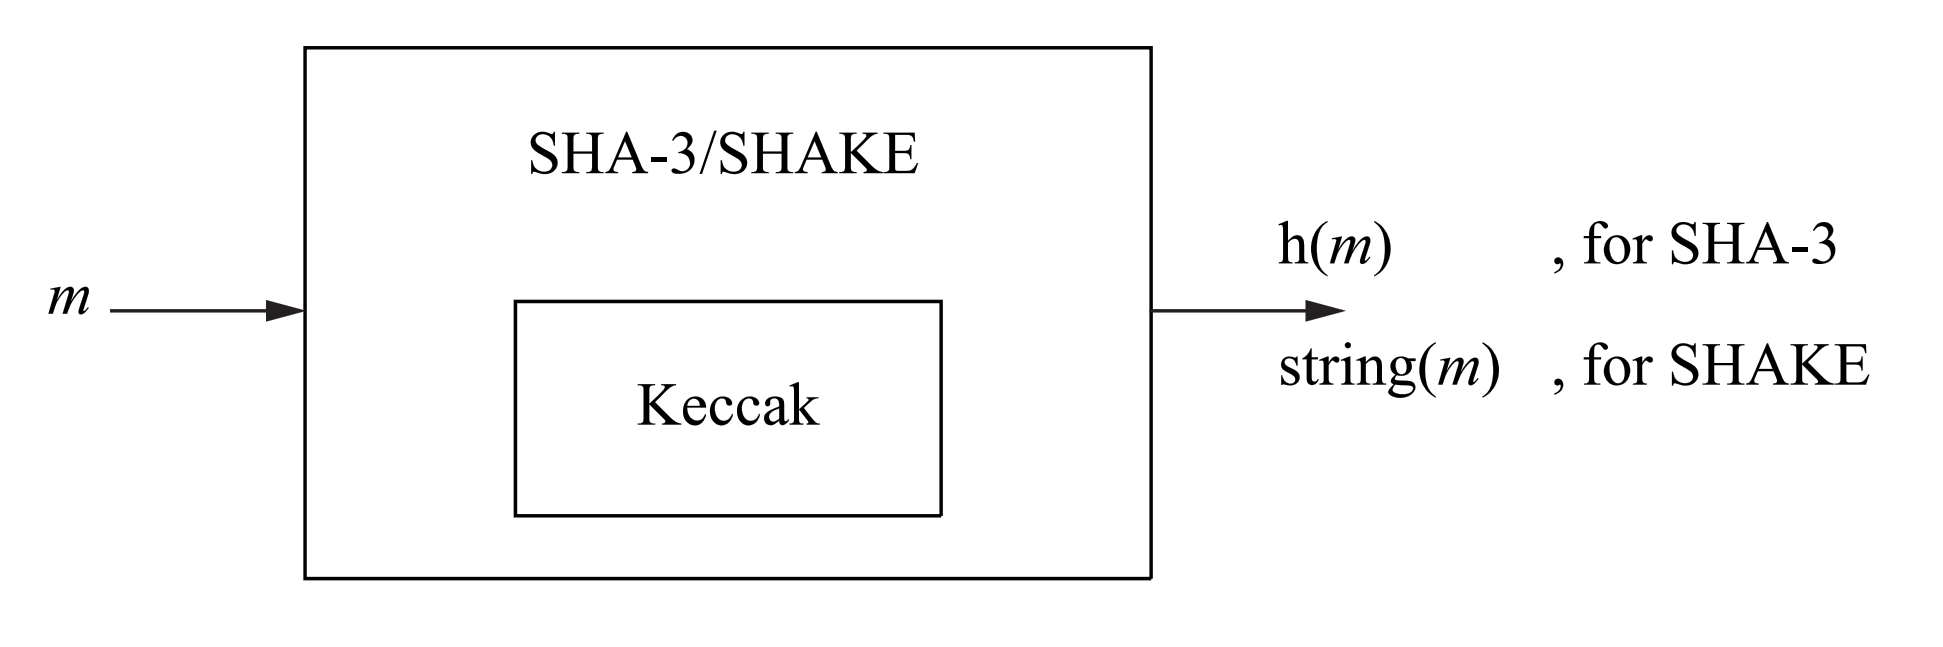
\includegraphics[width=\linewidth]{img/sha3_high.png}
\end{frame}

\begin{frame}{Keccak: Construção Esponja (Visão Geral)}
  \begin{itemize}
    \item \textbf{SHA-3} e as variantes \textbf{SHAKE128/256} são baseadas no algoritmo \textbf{Keccak}.
    \item SHA-3:
      \begin{itemize}
        \item Recebe uma mensagem $m$.
        \item Produz um \textbf{digest de tamanho fixo} $h(m)$.
      \end{itemize}
    \item SHAKE128/256 (\textit{Secure Hash Algorithm Keccak}):
      \begin{itemize}
        \item São \textbf{funções de saída extensível (XOF)}.
        \item Geram uma \textbf{string de bits de tamanho arbitrário} $\text{string}(m)$.
      \end{itemize}
    \item Keccak é baseado em uma \textbf{construção esponja}:
      \begin{itemize}
        \item Antes de tudo, há um \textbf{preprocessamento} de $m$ (sufixo + padding, divisão em blocos).
        \item Depois disso, a esponja possui duas fases:
          \begin{enumerate}
            \item \textbf{Fase de absorção}: processa os blocos de entrada $x_i$.
            \item \textbf{Fase de espremer (squeezing)}: gera blocos de saída $y_j$.
          \end{enumerate}
      \end{itemize}
    \item Keccak, por si só, permite gerar \textbf{quantos blocos de saída $y_j$ forem necessários}:
      \begin{itemize}
        \item Para \textbf{SHA-3}: apenas $y_0$ é usado, e seus primeiros bits formam $h(m)$.
        \item Para \textbf{SHAKE128/256}: usa-se a sequência $y_0, y_1, \dots$ conforme a aplicação.
      \end{itemize}
  \end{itemize}
\end{frame}

\begin{frame}{Keccak: Construção Esponja}
    \begin{figure}
        \centering
        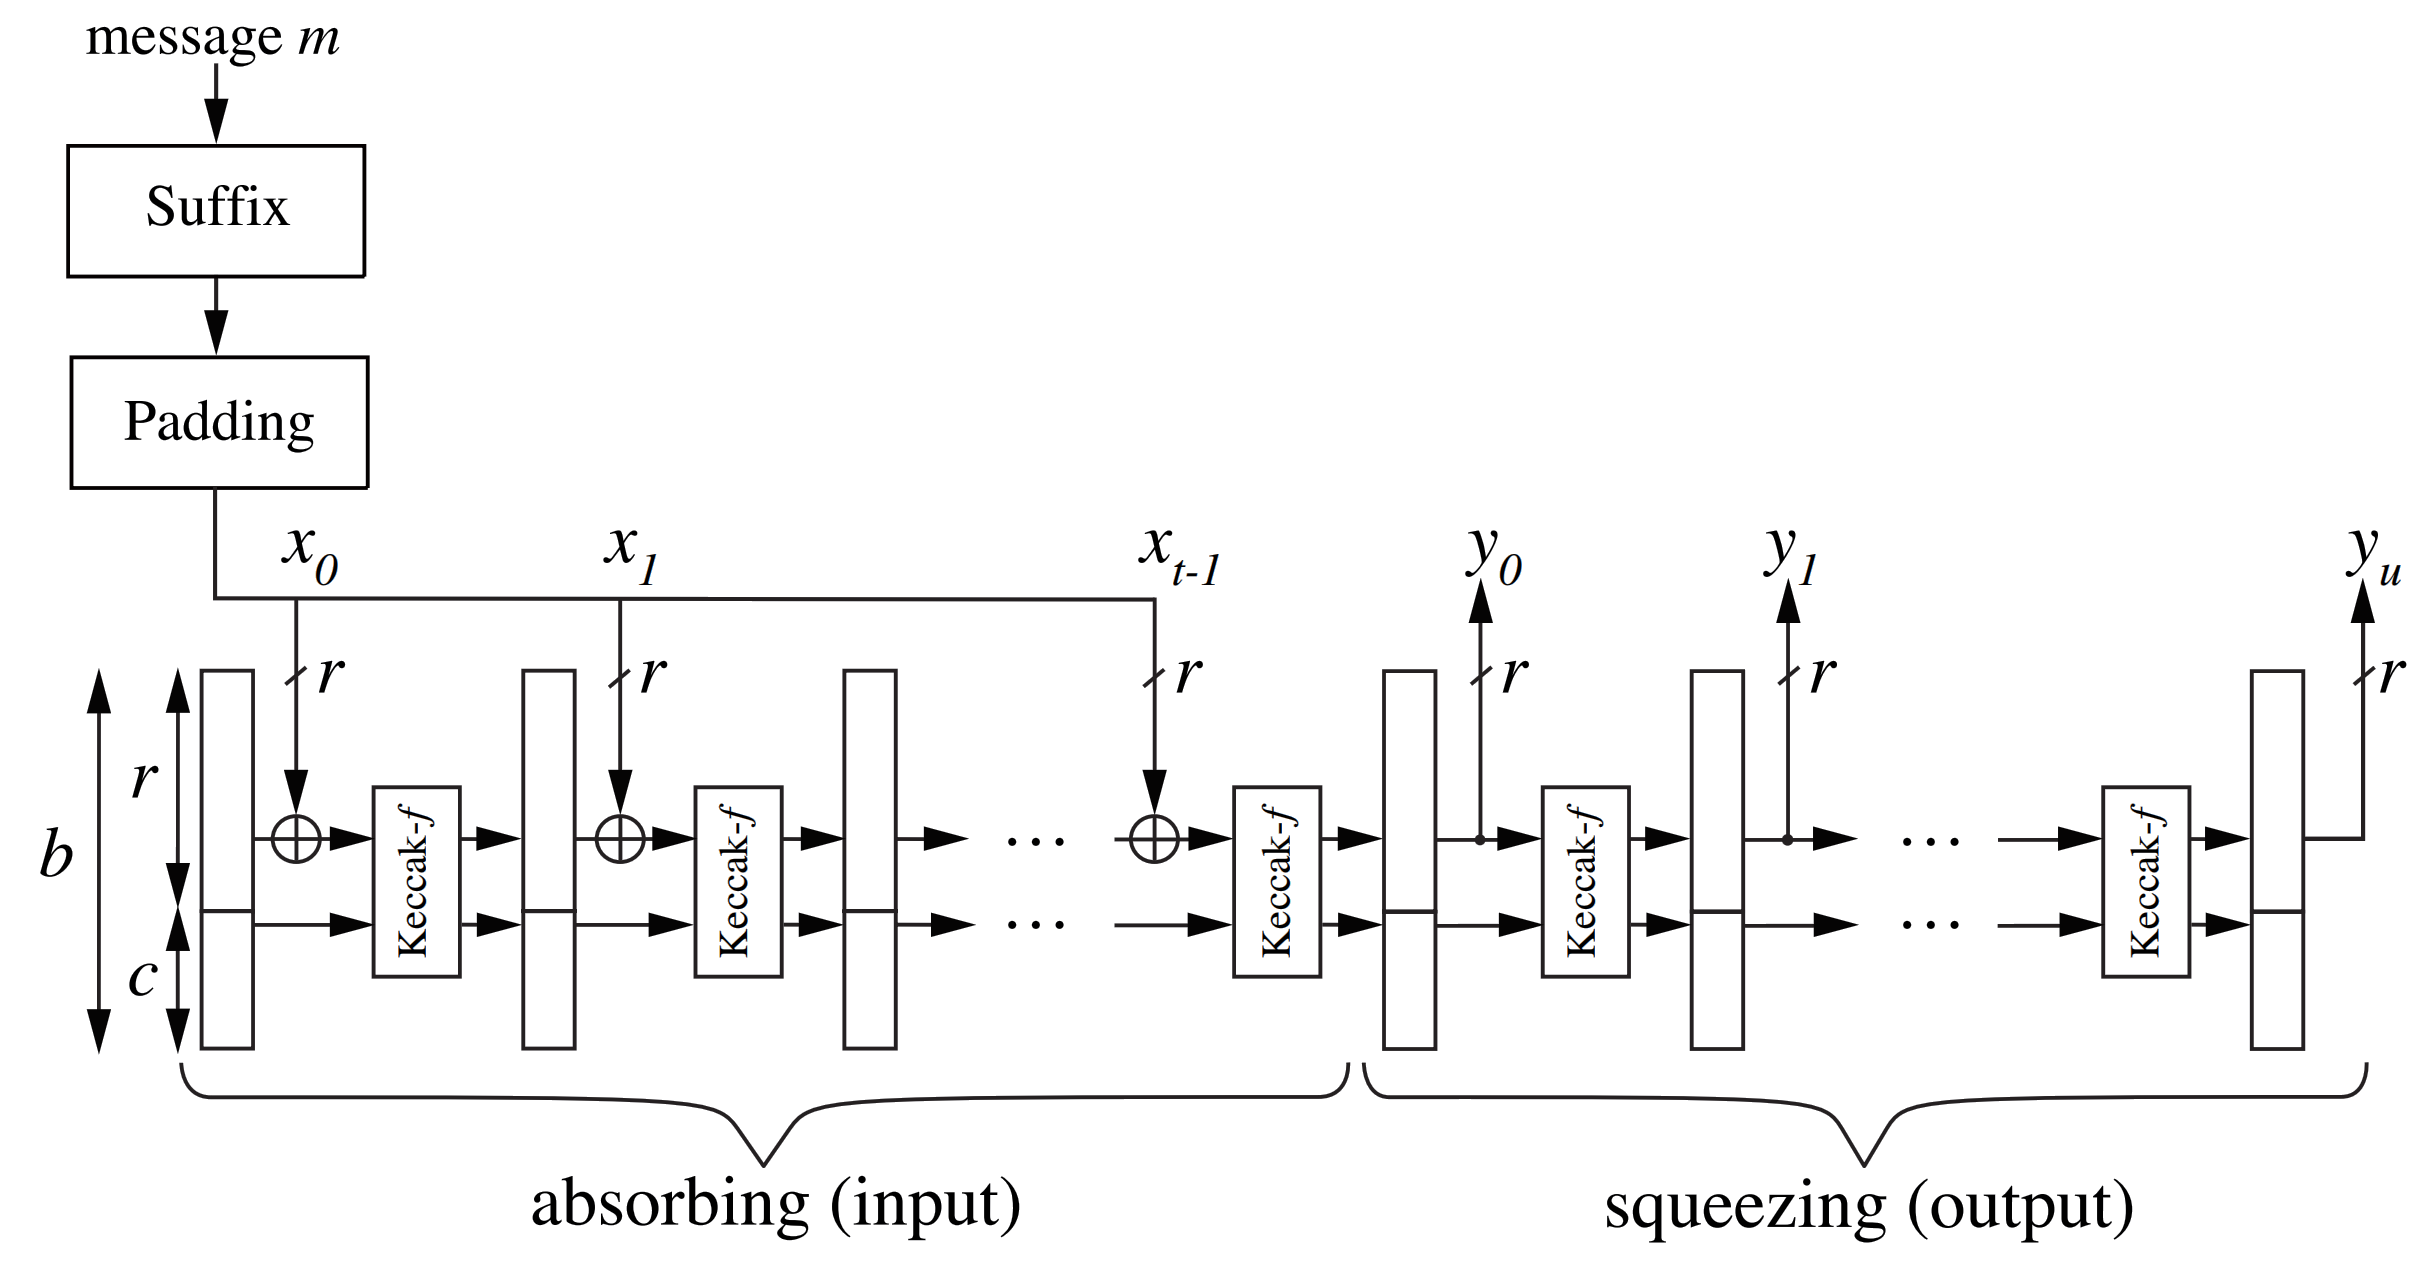
\includegraphics[width=1\linewidth]{img/keccak_construction.png}
    \end{figure}
\end{frame}

\begin{frame}{Parâmetros da Esponja Keccak: \texorpdfstring{$b$, $r$, $c$}{b, r, c}}
  \begin{itemize}
    \item O “coração” é a função de permutação \textbf{Keccak-f}.
    \item Keccak-f opera sobre um \textbf{estado interno} de largura $b$ bits:
      \[
        b = r + c
      \]
      onde:
      \begin{itemize}
        \item $b$ é a \textbf{largura do estado} (fixada em $b = 1600$ bits).
        \item $r$ é a \textbf{taxa de bits (bit rate)}:
          \begin{itemize}
            \item comprimento de cada bloco de mensagem $x_i$;
          \end{itemize}
        \item $c$ é a \textbf{capacidade}:
          \begin{itemize}
            \item controla o \textbf{nível de segurança} da construção.
          \end{itemize}
      \end{itemize}
    \item Diferentes combinações de $(r,c)$, com $b = 1600$ fixo, resultam em:
      \begin{itemize}
        \item diferentes \textbf{desempenhos} (mais/menos bits absorvidos/expelidos por chamada de Keccak-f);
      \end{itemize}
  \end{itemize}

    \begin{figure}
        \centering
        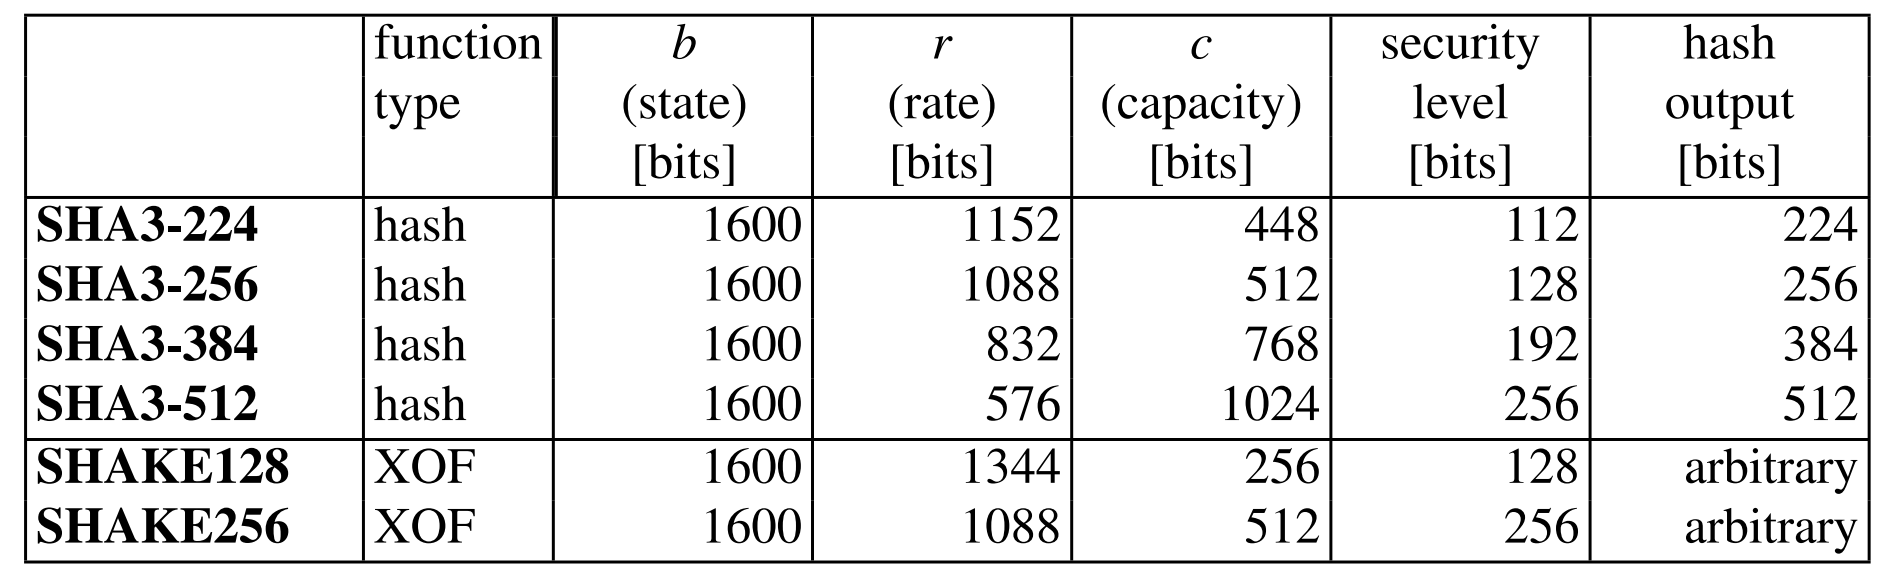
\includegraphics[width=0.65\linewidth]{img/parametersSHA3.png}
    \end{figure}
  
\end{frame}

\begin{frame}{SHA-3 / SHAKE: Sufixo e Padding}
  \begin{itemize}
    \item Antes do processamento de uma mensagem $m$, são aplicados:
      \begin{itemize}
        \item um \textbf{sufixo} específico de SHA-3 ou SHAKE;
        \item um \textbf{padding} definido na especificação de Keccak.
      \end{itemize}
    \item O sufixo \textbf{não} faz parte da função Keccak em si, mas é exigido por SHA-3 e SHAKE128/256:
      \begin{itemize}
        \item SHA-3: \quad $\text{suf} = \texttt{01}$;
        \item SHAKE128/256: \quad $\text{suf} = \texttt{1111}$.
      \end{itemize}
    \item Esses sufixos diferentes garantem \textbf{separação de domínio}:
      \begin{itemize}
        \item a mesma mensagem $m$ não produz a mesma sequência de bits
              quando usada em SHA-3 e em SHAKE;
        \item evita reutilização insegura do mesmo estado interno para funções com propósitos diferentes
              (hash fixo vs XOF/pseudorrandômico).
      \end{itemize}
    \item Após anexar o sufixo, aplica-se o \textbf{multi-rate padding}:
      \[
        \text{pad}(m,\text{suf}) = m \,\|\, \text{suf} \,\|\, \texttt{10}^*\texttt{1}
      \]
        onde:
        \begin{itemize}
        \item $\texttt{10}^*\texttt{1}$ é uma sequência que começa com \texttt{1},
              segue com o menor número possível de zeros e termina com \texttt{1};
        \item o objetivo é que o comprimento total seja um múltiplo de $r$ bits.
      \end{itemize}
  \end{itemize}
\end{frame}

\begin{frame}{SHA-3 / SHAKE: Comprimento da Saída e Uso de \texorpdfstring{$y_j$}{yj}}
  \begin{itemize}
    \item Após absorver todos os blocos de entrada $x_i$, Keccak entra na fase de \textbf{squeezing},
          gerando blocos de saída $y_0, y_1, \dots$, cada um com $r$ bits.
    \item \textbf{SHA-3}:
      \begin{itemize}
        \item Apenas o \textbf{primeiro bloco} $y_0$ é considerado.
        \item $y_0$ tem $r$ bits, mas o digest requerido é de 224, 256, 384 ou 512 bits.
        \item Usa-se apenas os \textbf{bits mais significativos} de $y_0$;
              os demais bits de $y_0$ são descartados.
      \end{itemize}
    \item \textbf{SHAKE128/256}:
      \begin{itemize}
        \item Todos os $r$ bits de $y_0$ podem ser usados.
        \item Se a aplicação necessita de mais que $r$ bits:
          \begin{itemize}
            \item aplica-se a permutação \textbf{Keccak-f} novamente ao estado;
            \item gera-se $y_1, y_2, \dots$ até alcançar o comprimento desejado.
          \end{itemize}
        \item Isso transforma SHAKE em uma \textbf{XOF}: função de saída extensível, útil como
              hash configurável, KDF ou PRNG.
      \end{itemize}
    \item O tamanho de padding:
      \begin{itemize}
        \item mínimo: sequência \texttt{11} (2 bits);
        \item máximo: padrão \texttt{10...01} com comprimento $r+1$ bits.
      \end{itemize}
  \end{itemize}
\end{frame}



\begin{frame}{Função Keccak-f: Permutação Base de SHA-3}
  \begin{itemize}
    \item \textbf{Keccak-f} é o núcleo de \textbf{Keccak}, logo de \textbf{SHA-3} e \textbf{SHAKE128/256}.
    \item É uma \textbf{permutação} sobre $2^b$ estados:
      \begin{itemize}
        \item Cada inteiro de $b$ bits é mapeado \emph{bijetivamente} em outro inteiro de $b$ bits.
      \end{itemize}
    \item O estado é visto como um arranjo 3D de bits:
      \[
        b = 5 \times 5 \times w
      \]
      \begin{itemize}
        \item Coordenadas $(x,y)$ formam uma \textbf{coluna}, e os $w$ bits ao longo de $z$ são chamados de \textbf{lane}.
        \item Para SHA-3/SHAKE: $w = 64$ bits é mapeado para: $b = 1600$ bits.
      \end{itemize}
    \item O estado de 1600 bits encaixa bem em arquiteturas de 64 bits:
      \begin{itemize}
        \item Pode ser armazenado como um vetor de 25 palavras de 64 bits.
      \end{itemize}
  \end{itemize}
\end{frame}

\begin{frame}{Keccak-f: Tamanhos de Estado e Estrutura de Rodadas}
  \begin{itemize}
    \item Keccak-f suporta sete tamanhos de estado:
      \[
        b = 25 \cdot 2^l,\ \ l = 0,1,\dots,6
      \]
      \[
        w = 2^l,\quad b = 5 \times 5 \times w
      \]
    \item Número de rodadas para cada $b$:
      \[
        n_r = 12 + 2^l
      \]
      \begin{itemize}
        \item Para SHA-3/SHAKE128/256: $b = 1600$, $w = 64$, $l = 6$, logo $n_r = 24$.
      \end{itemize}
    \item Cada rodada de Keccak-f aplica, em sequência, cinco transformações lineares/não lineares:
      \[
        \theta,\ \rho,\ \pi,\ \chi,\ \iota
      \]
      \vspace{-1.5em}
      \begin{itemize}
        \item Todas as rodadas têm a mesma estrutura.
        \item Diferem apenas pela \textbf{constante de rodada} $RC[i]$, usada na etapa $\iota$.
      \end{itemize}
    \item Essência: uma permutação altamente misturadora de 1600 bits, aplicada várias vezes, que confere à esponja Keccak suas propriedades de segurança.
  \end{itemize}
\end{frame}



\begin{frame}{Visualização do estado interno}

    Visualização 3D do estado do Keccak, cada pequeno cubo representa um bit. 
    Para o SHA-3 e o SHAKE128/256, a “profundidade” do arranjo ao longo do eixo $z$ é $w = 64$.
    \begin{figure}
        \centering
        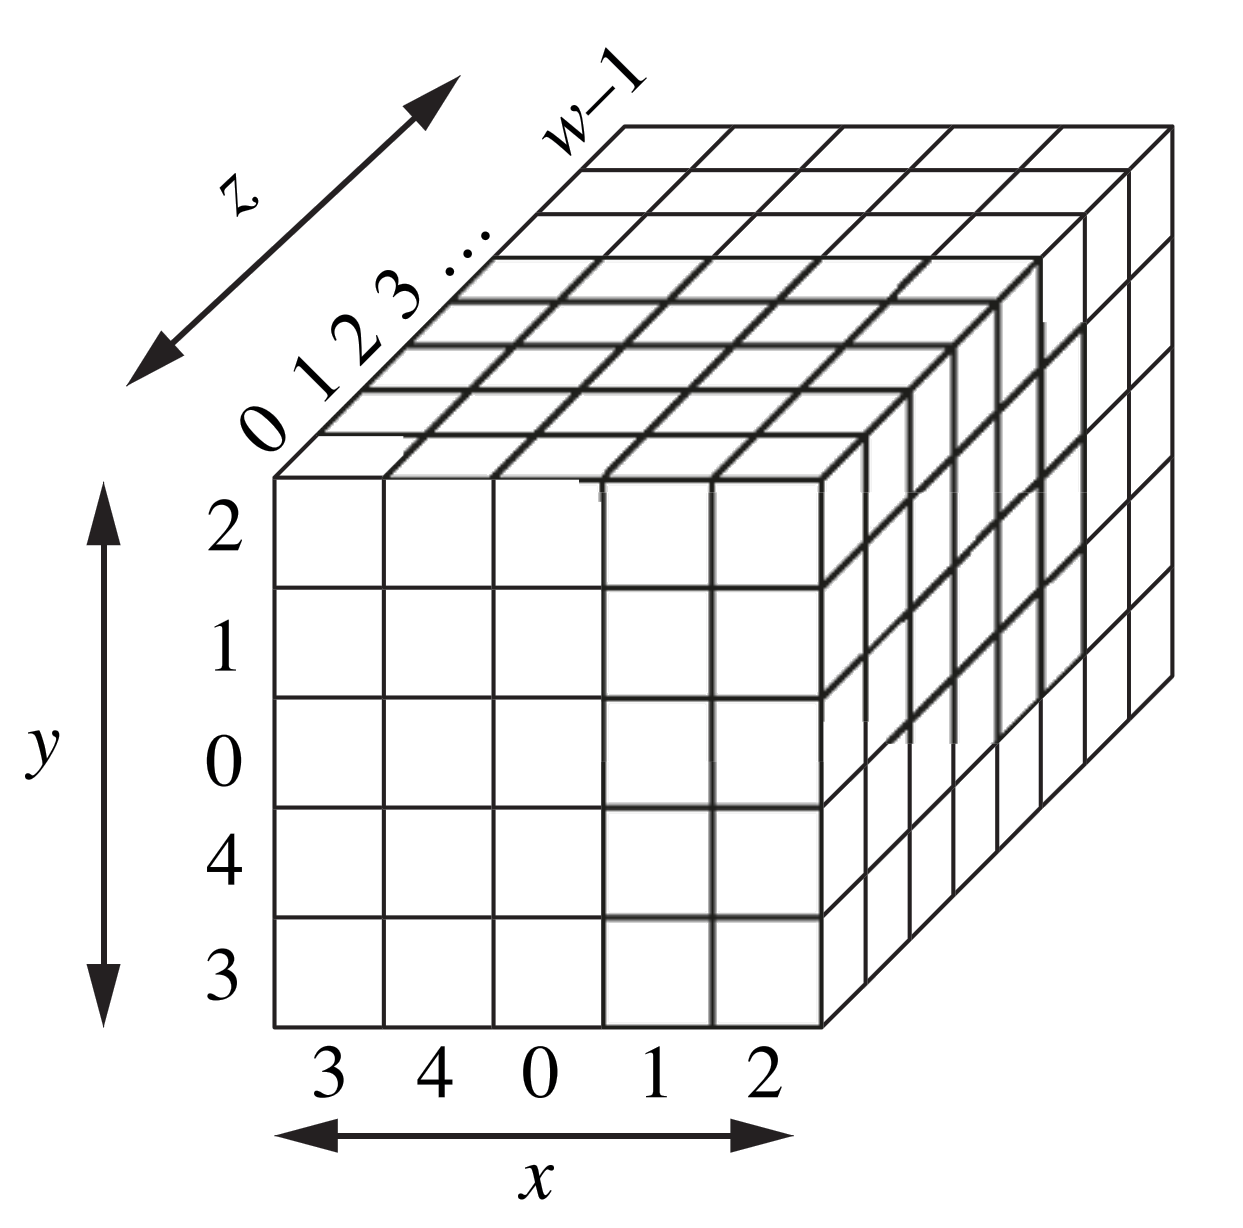
\includegraphics[width=0.3\linewidth]{img/state.png}
    
    \end{figure}

    Os diferentes tamanhos de estado e o número de rodadas de Keccak-f; note que $b = 1600$ e $n_r = 24$ para o SHA-3 e o SHAKE128/256.

    \begin{figure}
        \centering
        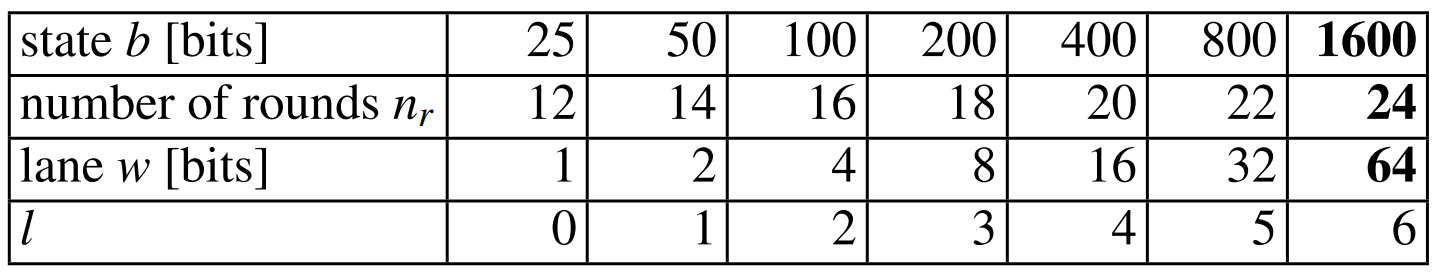
\includegraphics[width=0.5\linewidth]{img/states_table.png}
    \end{figure}
        
\end{frame}


\begin{frame}{Estrutura Interna da Função Keccak-\textit{f}}
\begin{itemize}
  \item Cada chamada de Keccak-f aplica $n_r = 24$ rodadas idênticas, e cada rodada é composta em série pelas etapas $\theta$, $\rho$, $\pi$, $\chi$ e $\iota$; apenas a etapa $\iota$ recebe uma constante de rodada $RC[i]$ diferente em cada iteração.
\end{itemize}
    \begin{figure}
        \centering
        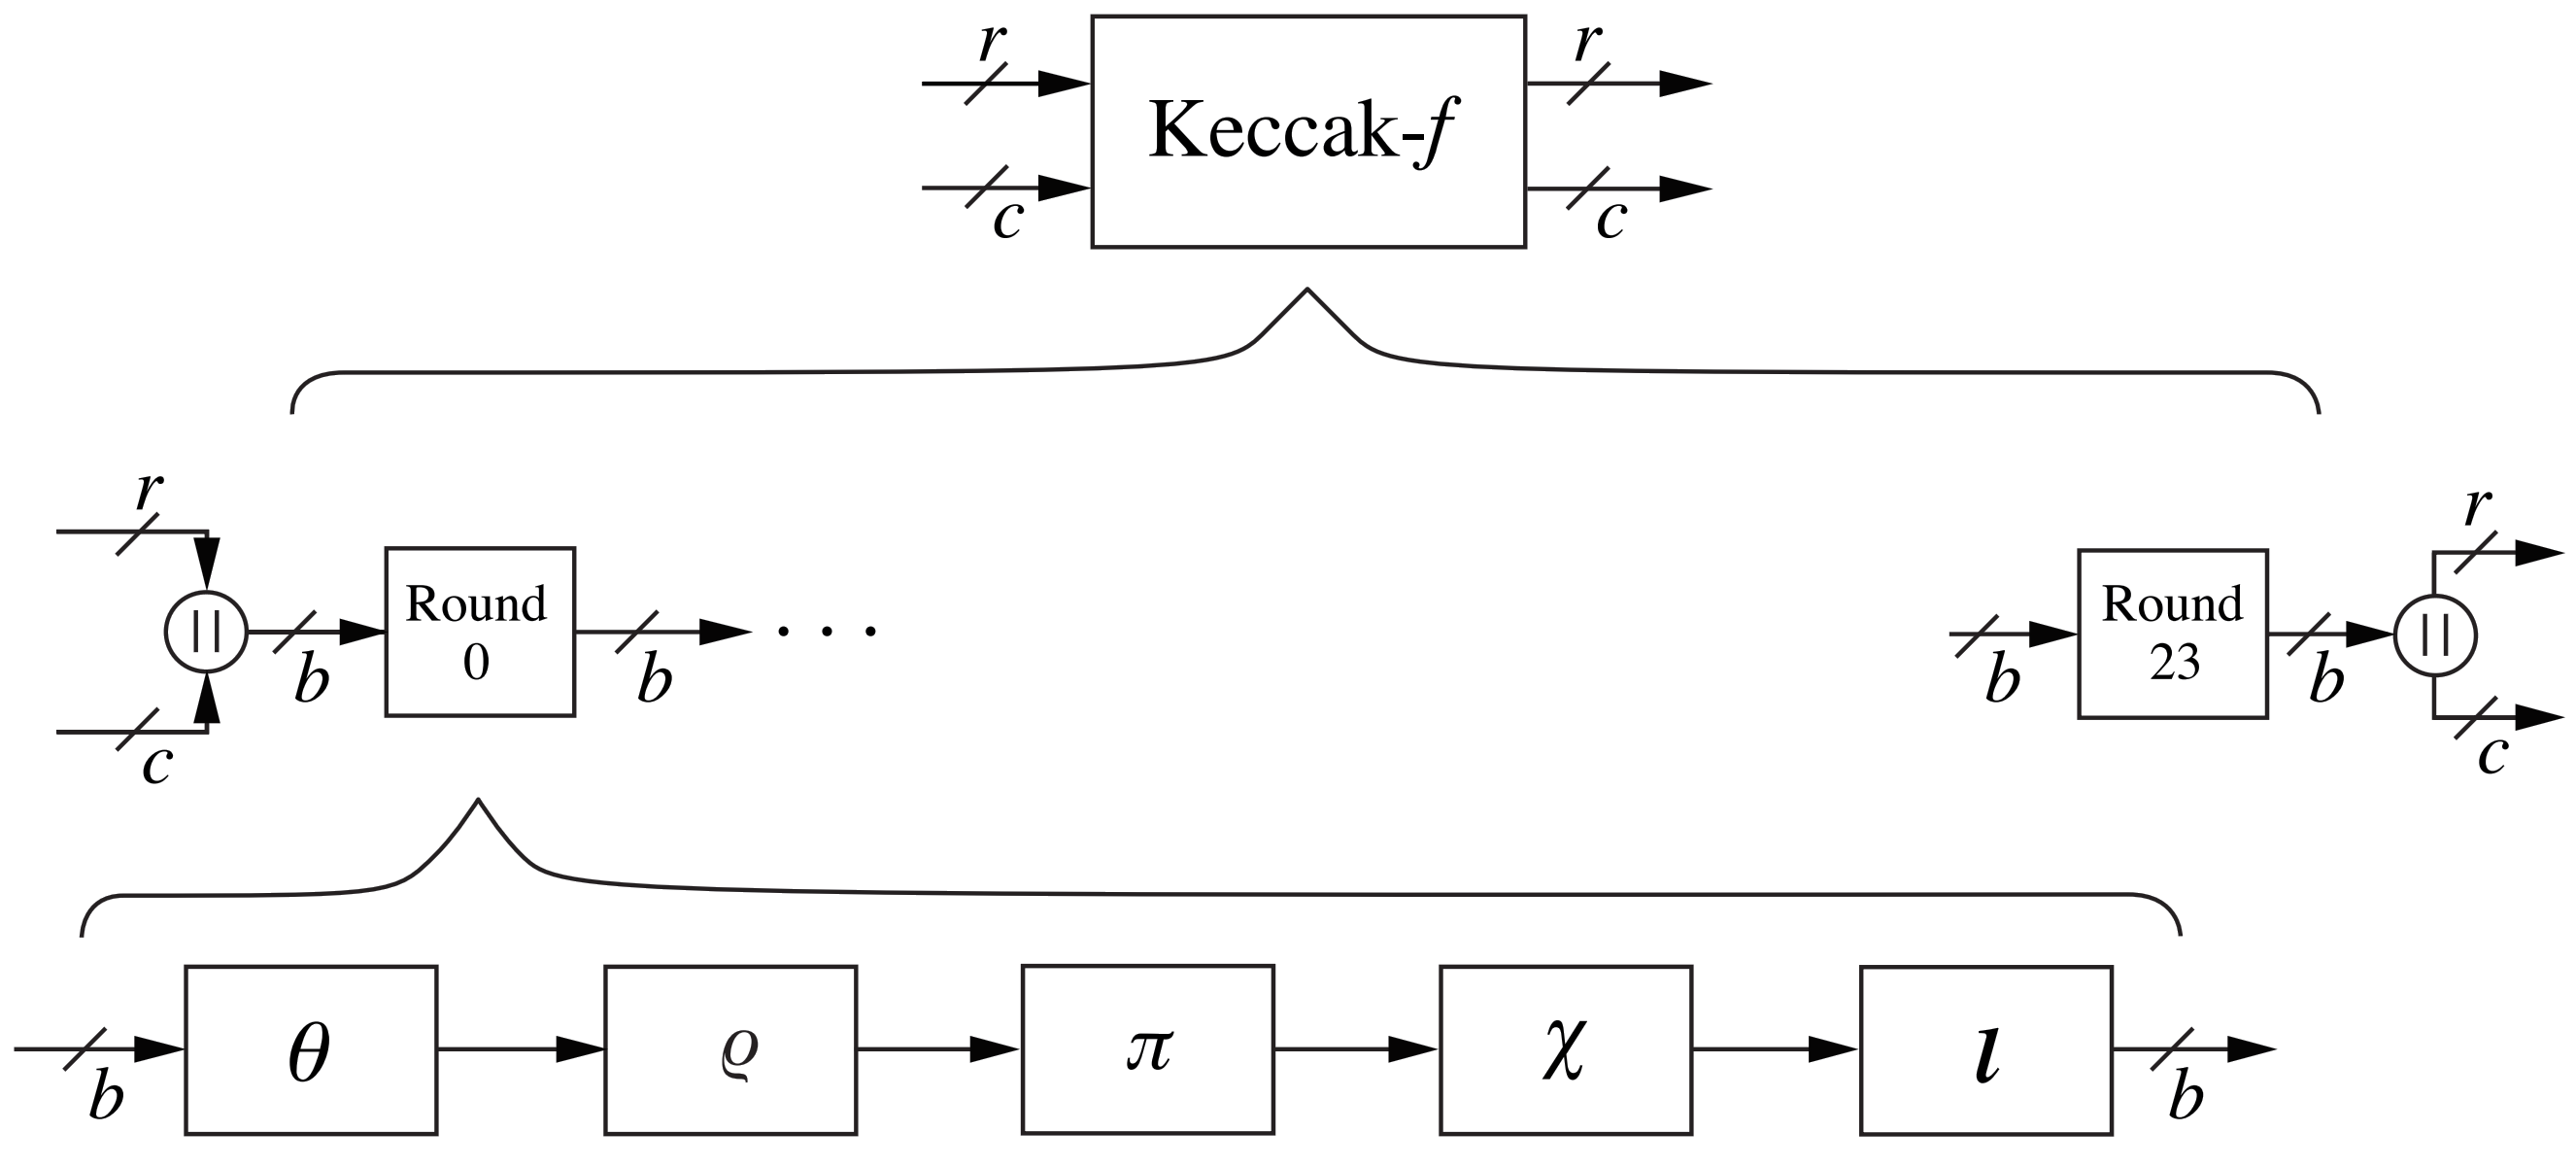
\includegraphics[width=0.7\linewidth]{internal_f_function.png}
    \end{figure}
    
\end{frame}


\begin{frame}{Etapa $\theta$ do Keccak-f}
  \begin{columns}
    \begin{column}{0.65\textwidth}
      \begin{itemize}
        \item Transformação linear de difusão do Keccak-f: cada bit do estado é substituído pelo XOR entre si e com outros 10 bits de sua vizinhança, espalhando a influência de cada coluna por todo o estado.
        \item Na implementação, calculam-se:
        \begin{itemize}
            \item $C[x] = A[x,0]\oplus A[x,1]\oplus A[x,3] \oplus A[x,4]$
            \item $D[x] = C[x-1] \oplus \text{rot}(C[x+1],1)$
            \item $A'[x,y] = A[x,y] \oplus D[x]$
        \end{itemize}
      \end{itemize}
    \end{column}
    \begin{column}{0.35\textwidth}
        \begin{figure}
            \centering
            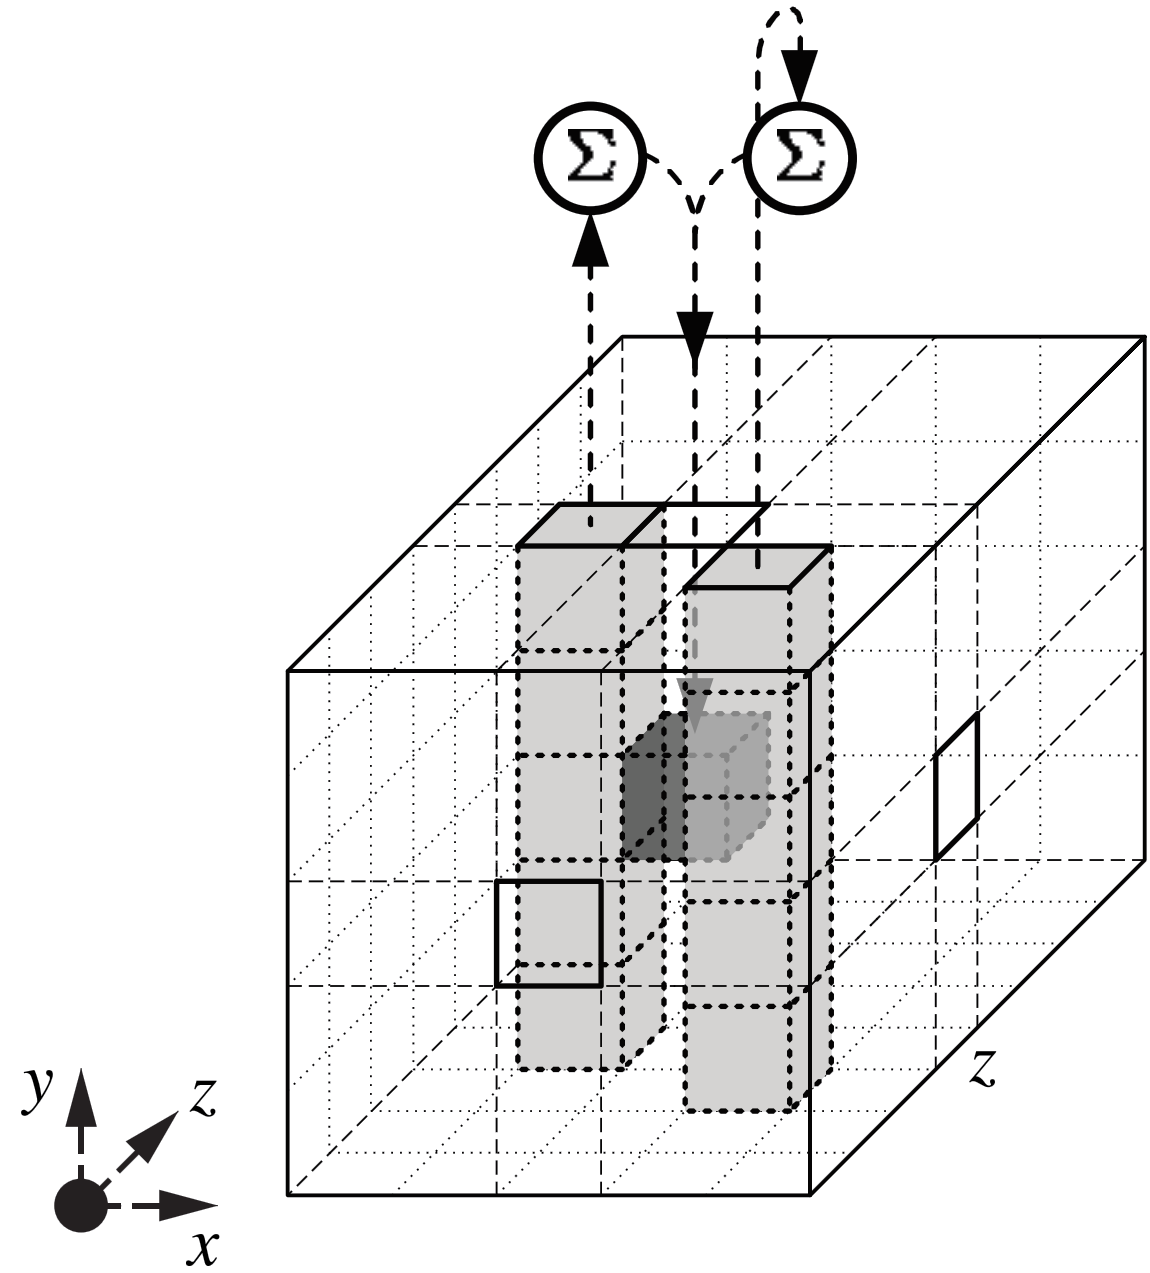
\includegraphics[width=1\linewidth]{img/theta.png}
        \end{figure}
    \end{column}
  \end{columns}
\end{frame}

\begin{frame}{Etapa $\rho$ do Keccak-f}
  \begin{itemize}
    \item O estado é visto como um arranjo $5 \times 5$ de \emph{lanes} $A(x,y)$, cada um com $w$ bits (para o SHA3 e SHAKE128/256 $w = 64$).
    \item Cada lane é submetida a uma \textbf{rotação circular de bits} com um deslocamento (offset) específico, que depende exclusivamente das coordenadas $(x,y)$ dessa lane.
    \item Todos os deslocamentos são tomados módulo $w$, e foram escolhidos de forma a espalhar os bits ao longo da dimensão $z$, contribuindo para uma boa difusão em combinação com as demais etapas da permutação.
    \item A tabela abaixo mostra, para cada posição $(x,y)$, o número de bits de rotação aplicado na etapa $\rho$.
  \end{itemize}
  \centering
  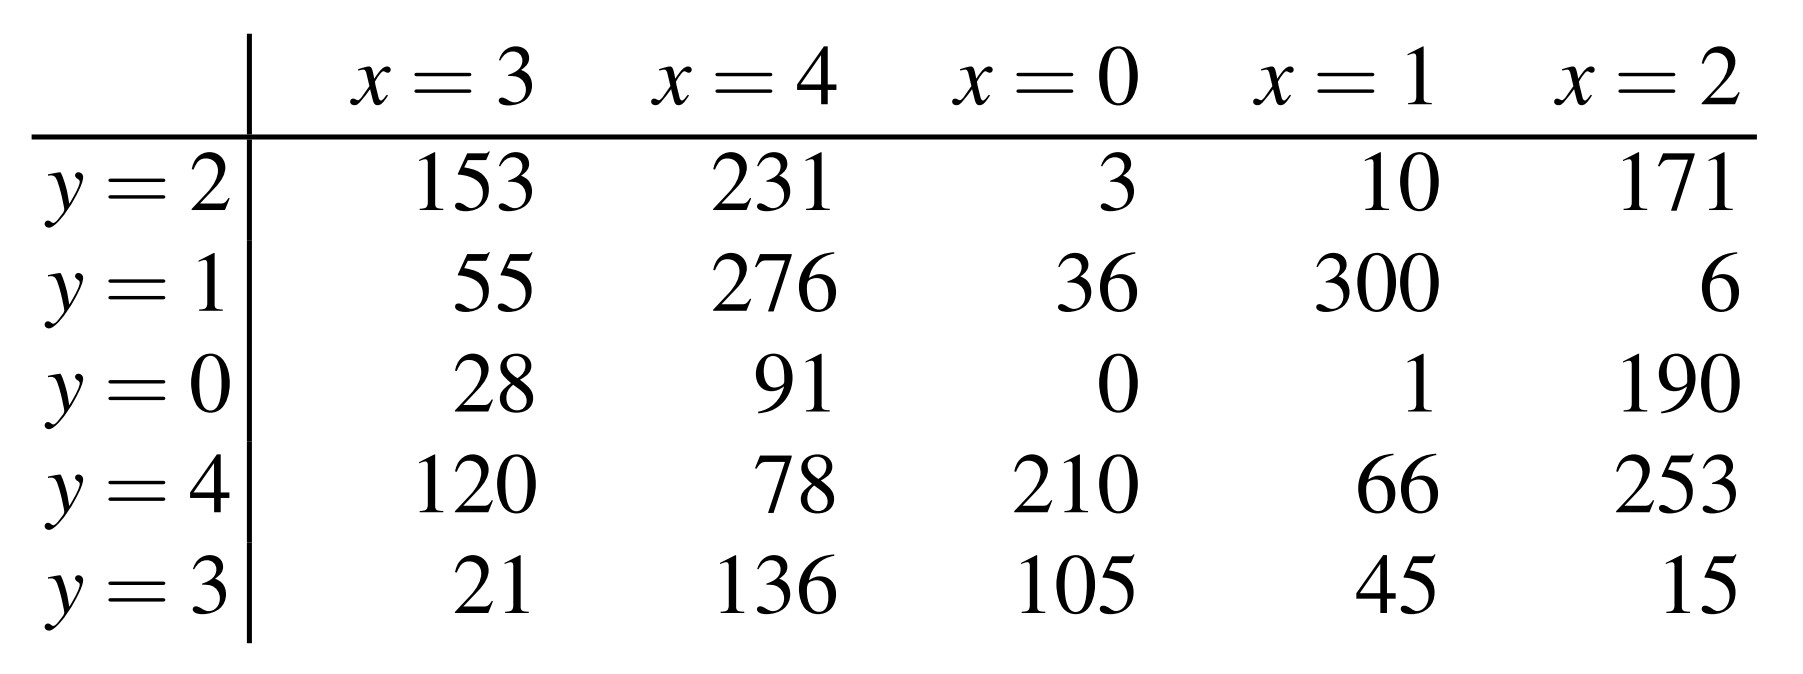
\includegraphics[width=0.5\linewidth]{rho_table.png}
\end{frame}

\begin{frame}{Etapa $\pi$ do Keccak-f}
  \begin{itemize}
    \item A etapa $\pi$ é uma \textbf{permutação das 25 lanes} do estado $A(x,y)$ visto como uma matriz $5 \times 5$.
    \item Dado o novo arranjo $A'$, a regra de permutação é:
      \[
        A'[x,y] = A[x + 3y,\, x] \,, \quad x,y = 0,1,2,3,4
      \]
      onde todas as coordenadas são computadas módulo $5$.
    \item Nenhum bit é modificado, apenas \textbf{reordenado}:
      \begin{itemize}
        \item a etapa $\pi$ redistribui as lanes no plano $(x,y)$;
        \item prepara o estado para que as operações seguintes (especialmente a $\chi$) combinem bits de posições que antes não interagiam.
      \end{itemize}
    \item Exemplo: a posição $A'[2,3]$ será preenchida pela lane
      \[
        A[2 + 3 \cdot 3,\, 2] = A[11,2] = A[1,2] \quad (\text{mód } 5),
      \]
      isto é, a lane originalmente em $(1,2)$ é movida para a borda inferior direita.
  \end{itemize}
\end{frame}

\begin{frame}{Etapa $\chi$ do Keccak-f}
  \begin{itemize}
    \item \textbf{Única operação não linear} dentro do Keccak-f.
    \item Opera por linhas de lanes: para cada coordenada $(x,y)$ temos
      \[
        A'[x,y] = A[x,y] \oplus \bigl( \overline{A[x+1,y]} \land A[x+2,y] \bigr),
        \quad x,y = 0,1,2,3,4
      \]
      onde os índices são tomados módulo $5$.
  \end{itemize}

  \begin{figure}
      \centering
      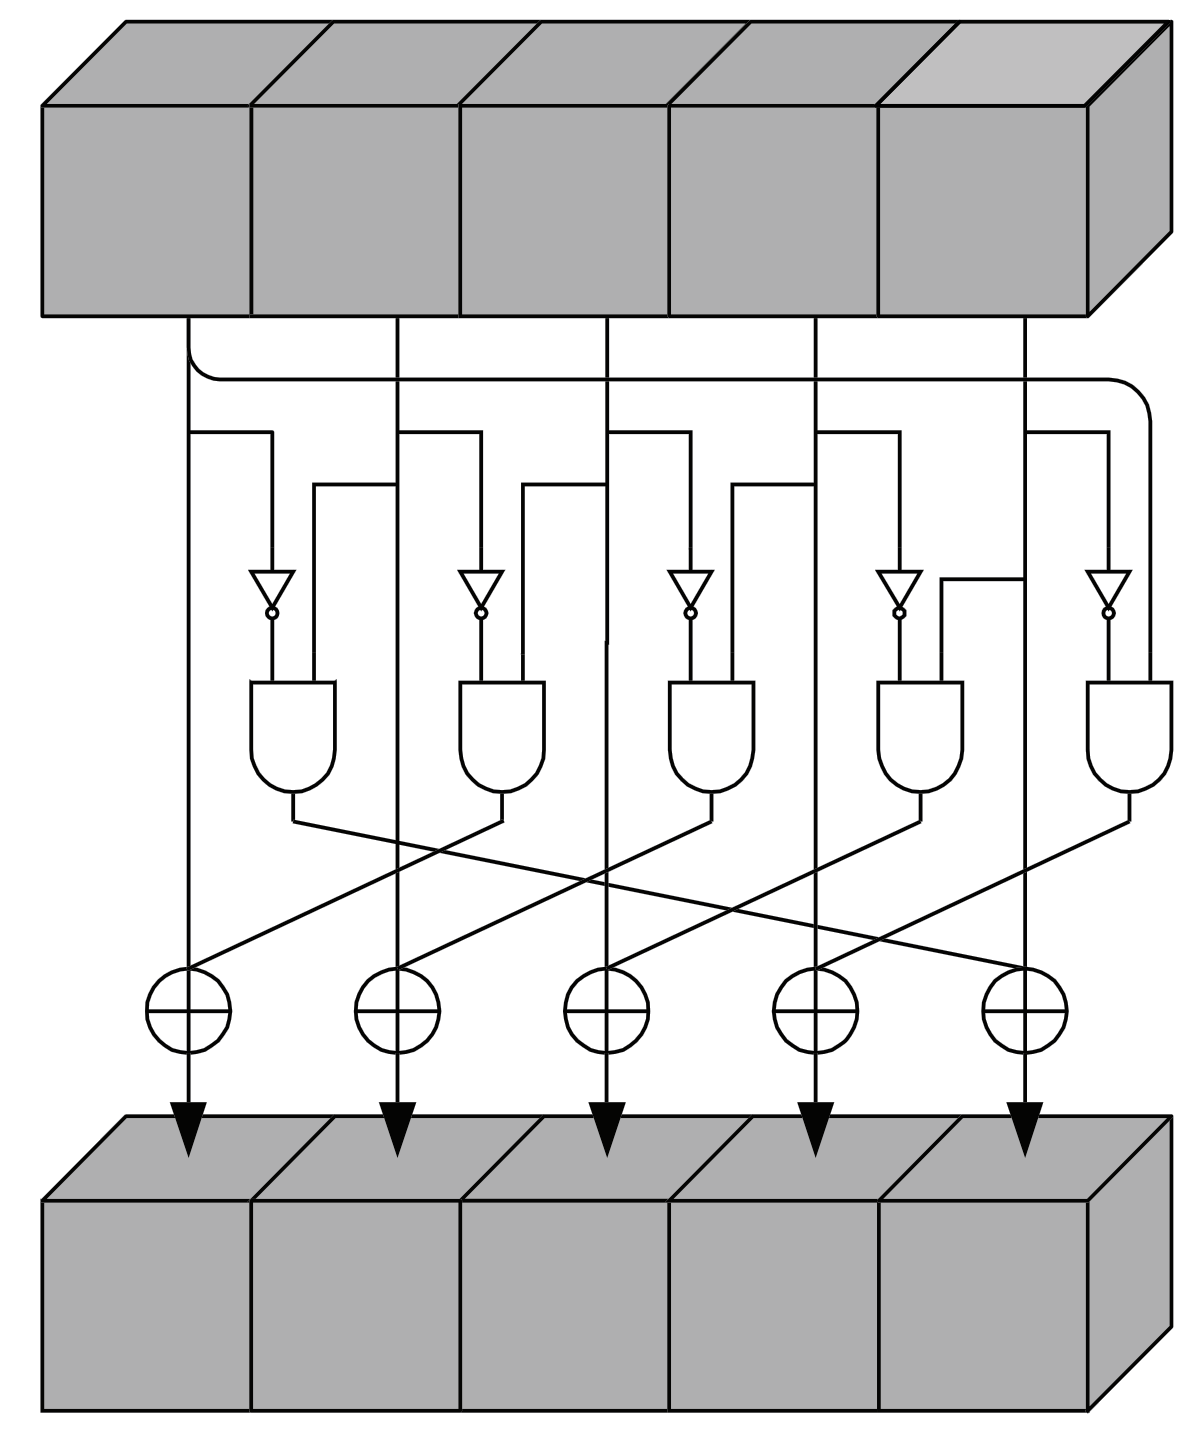
\includegraphics[width=0.35\linewidth]{img/xi_step.png}
  \end{figure}
\end{frame}


\begin{frame}{Etapa $\iota$ do Keccak-f}
  \begin{itemize}
    \item A etapa $\iota$ adiciona uma \textbf{constante de rodada} de $w$ bits à lane na posição $(0,0)$ do estado:
      \[
        A'[0,0] = A[0,0] \oplus RC[i].
      \]
    \item A constante $RC[i]$ depende da rodada $i$:
      \begin{itemize}
        \item o número de rodadas $n_r$ varia com o parâmetro $b$;
        \item para SHA-3 e SHAKE128/256 temos $n_r = 24$ rodadas, logo $RC[0],\dots,RC[23]$.
      \end{itemize}
    \item Cada $RC[i]$ é, em essência, um vetor quase todo nulo, com bits pseudoaleatórios em posições específicas (por exemplo 1, 2, 3, 7, 15, 31, 63), gerados por um LFSR de grau 8.
    \item A função da etapa $\iota$ é \textbf{quebrar simetrias} entre rodadas: ela insere dependência explícita do índice de rodada na permutação Keccak-f, reforçando a segurança contra ataques estruturais.
  \end{itemize}
\end{frame}


\begin{frame}{Lições Aprendidas sobre Funções Hash}
  \begin{itemize}
    \item Funções hash são \textbf{sem chave} (keyless) e têm muitas aplicações em sistemas de segurança modernos, como \textbf{assinaturas digitais} e \textbf{MACs}.
    \item As três propriedades de segurança fundamentais são:
      \begin{itemize}
        \item \textbf{one-wayness} (pré-imagem difícil),
        \item \textbf{segunda pré-imagem} difícil,
        \item \textbf{resistência a colisões}.
      \end{itemize}
    \item Para resistir a ataques de colisão, a saída de uma função hash deve ter, em geral, \textbf{256 bits ou mais}.
    \item \textbf{SHA-2} e \textbf{SHA-3} são considerados altamente seguros atualmente; não há ataques práticos conhecidos. Já o \textbf{SHA-1} é considerado inseguro.
    \item Além de algoritmos dedicados (como SHA-2 e SHA-3), é possível construir funções hash a partir de \textbf{cifras de bloco}.
    \item \textbf{SHA-3} baseia-se em uma \textbf{construção esponja}, o que o torna, internamente, bem diferente de SHA-1 e SHA-2.
    \item Em \textbf{hardware}, SHA-3 tende a ser mais eficiente, sendo adequado para aplicações móveis e embarcadas; em \textbf{software}, SHA-2 costuma ser mais rápido do que SHA-3.
  \end{itemize}
\end{frame}


\end{document}
